\documentclass[oneside,11pt]{article}
\usepackage[algo,uml,french,url]{my_package}

\title{Parallélisation \& modèles\\de programmation}

\begin{document}
\begin{empfile}

\begin{empcmds}
input metauml;
\end{empcmds}

\maketitle

\tableofcontents

\newpage
\section{Produit matriciel}

\subsection{Enoncé}
\textit{Matrice: Décrire un algorithme PRAM pour le modèle EREW qui utilise $O(n^3)$ processeurs pour multiplier deux matrices de taille $n*n$.\footnote{$c_{ij} = \sum_{k=0}^n a_{ik} b_{kj}$: \url{http://fr.wikipedia.org/wiki/Produit_matriciel}}}

\subsection{Solution}
Une solution consisterait à diffuser dans un premier temps toutes les données des matrices à multiplier à chaque processus puis de faire le produit des matrices en prenant le soin que chaque processus utilise les données qui leur est propre.

\subsubsection{La diffusion}
En respectant le modèle EREW, les matrices $A$ et $B \in K_{n*n}$ sont copiées, dans un premier temps, $n$ fois dans les cubes $A'$ et $B' \in K_{n*n*n}$. Ceci permet de reserver une dimension du cube à un processus et éviter toute lecture concurrente.\\

L'algorithme \ref{diffusion} présente le pseudo-code de la fonction de diffusion qui prend comme donnée en entrée une matrice $M \in K_{n*n}$ et retourne un cube $M' \in K_{n*n*n}$ . Elle est exprimée en 2 étapes. La première consiste à affecter, en utilisant $O(n^2)$ processeurs, chaque point de la matrice dans la première dimension du cube. La deuxième effectue la copie en diffusion\footnote{Hot potato routing : \url{http://en.wikipedia.org/wiki/Hot_potato_routing}} de chaque point de la matrice situé à la première dimension du cube vers les autres dimensions du cube en utilisant $O(\log{n})$ processeurs et pour une matrice entière en $O(n^2 * \log{n})$.

\incmargin{1em}
\begin{algorithm}[here]
  \dontprintsemicolon
  \label{diffusion}
  \Donnees{$M \in K_{n*n}, n \in N$}
  \Res{$M' \in K_{n*n*n}$}
  \Deb{
    \textit{parallèle}\;
    \Pour{$i\leftarrow 0$ \KwA $n$}{
      \textit{parallèle}\;
      \Pour{$j\leftarrow 0$ \KwA $n$}{
        $m'(i,j,0)\leftarrow m(i,j)$
      }
    }

    \textit{parallèle}\;
    \Pour{$s\leftarrow 0$ \KwA $\log_2{n}$}{
      \textit{parallèle}\;
      \Pour{$h\leftarrow 0$ \KwA $s^2$}{
        \textit{parallèle}\;
        \Pour{$i\leftarrow 0$ \KwA $n$}{
          \textit{parallèle}\;
          \Pour{$j\leftarrow 0$ \KwA $n$}{
            $m'(i,j,2^s + h)\leftarrow m'(i,j,h)$
          }
        }
      }
    }
  }
  \caption{Copie de matrice en diffusion}
\end{algorithm}
\decmargin{1em}

\subsubsection{Le produit}

Toujours en respectant le modèle EREW, le produit matriciel prend en paramètre les cubes $A$ et $B \in K_{n*n*n}$ tel que chaque processus utilise sa dimension de cube respective pour lire les données de $a_{ij}$ et $b_{ij}$.\\

L'algorithme \ref{produit} présente le pseudo-code de la fonction de produit matriciel qui prend comme donnée en entrée les cubes $A$ et $B \in K_{n*n*n}$ et retourne une matrice $C \in K_{n*n}$. L'affectation des valeurs dans la matrice $C$ se fait en $O(n^2)$ et le produit de $c_{ij}$ se fait en $O(n)$.

\incmargin{1em}
\begin{algorithm}[here]
  \dontprintsemicolon
  \label{produit}
  \Donnees{$A,B \in K_{n*n*n}, n \in N$}
  \Res{$C \in K_{n*n}$}
  \Deb{
    \textit{parallèle}\;
    \Pour{$i\leftarrow 0$ \KwA $n$}{
      \textit{parallèle}\;
      \Pour{$j\leftarrow 0$ \KwA $n$}{
        $c(i,j)\leftarrow \sum_{k=0}^n a(i,k,p) * b(k,j,p)$
      }
    }
  }
  \caption{Produit matriciel}
\end{algorithm}
\decmargin{1em}

\subsubsection{L'implémentation}

Après avoir décrit la fonction de diffusion et le produit matriciel respectant tous deux le modèle EREW, nous allons voir l'implementation d'un produit de deux matrices $A$ et $B \in K_{n*n}$ produisant une troisième matrice $C \in K_{n*n}$.\\

L'algorithme \ref{implementation} décrit l'implémentation.

\incmargin{1em}
\begin{algorithm}[here]
  \dontprintsemicolon
  \label{implementation}
  \Donnees{$A,B \in K_{n*n}, n \in N$}
  \Res{$C \in K_{n*n}$}
  \Deb{
    $A'\leftarrow diffusion(A,n)$\;
    $B'\leftarrow diffusion(B,n)$\;
    $C\leftarrow produit(A',B')$\;
  }
  \caption{Implémentation du produit matriciel}
\end{algorithm}
\decmargin{1em}

%\newpage
\section{Découpage d'un tableau binaire}

\subsection{Énoncé}

\textit{Découpage d'un tableau : Soit $A$ un tableau de longueur $n$ dont les éléments sont soit des $0$ soit des $1$. Concevez un algorithme EREW de complexité $O(\log{n})$ utilisant $O(n)$ processeurs pour ranger tous les éléments $1$ à la droite du tableau tout en maintenant leur ordre relatif (propriété de stabilité des éléments).}

\textit{Hint : effectuer un calcul de préfixe pour déterminer quel devrait être la position de chaque élément.}

\subsection{Solution}

Notre tableau étant binaire, contenant que des $0$ et $1$, il devient facile de compter le nombre de $1$ en sommant toutes les valeurs du tableau pour ensuite déterminer à quel index placer les $0$ et $1$.

Toute fois pour respecter l'énoncé et avoir une complexité en $O(\log{n})$, nous allons devoir utiliser la fonction calculant la somme des préfixes.

\subsubsection{Déterminer l'index}

L'algorithme \ref{index} permet de déterminer l'index qui constituera la frontière entre les $0$ et $1$ dans le tableau. Pour cela il prend en paramètre le tableau binaire $B \in K_n$ ainsi que la taille du tableau $n \in N$.

\incmargin{1em}
\begin{algorithm}[here]
  \dontprintsemicolon
  \Donnees{$B \in K_n, n \in N$}
  \Res{$i \in N$}
  \Deb{
    $i\leftarrow {n - calcul\_somme\_prefixe(B)}$
  }
  \caption{Trouver l'index}
  \label{index}
\end{algorithm}
\decmargin{1em}

\subsubsection{Créer le tableau binaire}

L'algorithme \ref{creer_tableau_binaire} prend en paramètre l'index et la taille et crée un tableau binaire trié en fonction de l'index, $0$ à gauche et $1$ à droite.

\incmargin{1em}
\begin{algorithm}[here]
  \dontprintsemicolon
  \Donnees{$i,n \in N$}
  \Res{$B' \in K_n$}
  \Deb{
    \textit{parallèle}\;
    \Pour{$j\leftarrow 0$ \KwA $i$}{
      $B'(i)\leftarrow 0$
    }
    \textit{parallèle}\;
    \Pour{$j\leftarrow i$ \KwA $n$}{
      $B'(i)\leftarrow 1$
    }
  }
  \caption{Création du tableau binaire trié}
  \label{creer_tableau_binaire}
\end{algorithm}
\decmargin{1em}

\subsubsection{Implémentation}

L'algorithme \ref{decoupage} illustre la solution.

\incmargin{1em}
\begin{algorithm}[here]
  \dontprintsemicolon
  \Donnees{$B \in K_n$}
  \Res{$B' \in K_n$}
  \Deb{
    $i\leftarrow trouver\_index(B)$\;
    $B'\leftarrow creer\_tableau\_binaire(i)$\;
  }
  \caption{Découpage d’un tableau binaire}
  \label{decoupage}
\end{algorithm}
\decmargin{1em}

% \newpage
% %TODO
\section{Premier élément non-nul}
\subsection{Enoncé}
\textit{Premier élément non-nul : Soit $A$ un tableau de longueur $n$ dont les éléments sont soit des $0$ soit des $1$. Concevez un algorithme CRCW de complexit $O(1)$ qui utilise $O(n)$ processeurs.}

%\newpage
\section{Design}

Tous les exercices ont été developpés en C++ en utilisant le paradigme de programmation objet et le design qui suit a été élaboré pour regrouper les différents composants de calculs. Néanmoins une recherche a été effectué pour determiner les limites de OpenMP et C++. Il semblerait que les conteneurs fournit par la STL\footnote{Standard Template Library : \url{http://www.sgi.com/tech/stl/}} ne soient pas threadsafe\footnote{On dit qu’un programme ou qu'une portion de code est thread-safe s'il fonctionne correctement durant une exécution simultanée par plusieurs threads (processus légers). \url{http://fr.wikipedia.org/wiki/Threadsafe}}. Une étude\footnote{C++ and OpenMP : \url{http://www.compunity.org/events/pastevents/parco07/parco_cpp_openmp.pdf}} donne une liste non-exaustive des précautions à prendre lors de l’utilisation de OpenMP en C++. Cependant la version OpenMP 3.0 apporte des concepts nouveaux permettant l’utilisation notemment des iterateurs. On peut ainsi, par exemple, s’affranchir de simple indexeur de tableau et étendre la parallelisation sur des listes chainées.

\subsection{Diagramme de classes}

Deux grandes familles d'opérations coexistent. Les opérations de calcul à paramètre unique ``OMPComputeUnary'' et celles à deux paramètres ``OMPComputeBinary''. Tous deux renvoient un résultat. Elles sont préfixées de ``OMP'' pour OpenMP\footnote{Open Multi-Processing : http://openmp.org/}. Le calcul de somme des prefixes prenant un seul paramètre en entrée ``OMPVector'' et renvoyant un ``Atom'', cette classe se situe dans la famille ``OMPComputeUnary''. Le produit matriciel se situe, quant à lui, dans la famille “OMPComputeBinary”, cette classe prend deux paramètres ``OMPMatrix'' et retourne le même type. On peut imaginer d'autres opérations comme, par exemple, un produit vectoriel.

\subsection{Surcharge d'opérateur}

Compte tenu des possibilités offertes par le langage C++, comme la surcharge des opérateurs, l'opérateur $*$ se voit ainsi surchargé dans la classe ``OMPMatrix'' afin d'appeler implicitement la classe ``OMPMatrixProduct'' pour le calcul du produit matriciel. Ainsi en écrivant le code $C = A * B$ ceci revient à écrire $C = OMPMatrixProduct()(A, B)$.

%\newpage
\section{Mesure de performance}

Je profite de ce rapport pour parler d'un travail qui m'a été demandé en entreprise. Nous utilisons le framework EO\footnote{Evolving Object, \url{http://eodev.sf.net}} pour développer nos algorithmes évolutionnaires\footnote{Algorithme évolutionnaire : \url{http://fr.wikipedia.org/wiki/Algorithme_evolutionnaire}}. Le sujet consistait à implémenter, au framework EO, un parallélisme à mémoire partagée en utilisant OpenMP.

\subsection{Préambule}

Avant de commencer il est important de préciser que les EA\footnote{Algorithmes évolutionnaires} travaillent sur une population d'individu aussi appelé échantillon. Un individu étant représenté par un point dans l'échantillon, la complexité d'un problème est définit par le nombre de dimensions pour chaque individu.\\

Le problème est représenté par la fonction objectif qui prend en paramètre un individu (un point dans l'échantillon) et évalue toutes ses dimensions pour en déduire la qualité\footnote{Fitness en anglais}. La qualité est le critère de comparaison d'un point dans son échantillon.

\subsection{Identifier les ressources les plus utilisées}

Un test de profiling a été exécuté afin d'identifier les ressources les plus utilisées dans le framework EO. Le test nous a permit d'identifier une fonction qui est utilisée par une grande majorité des opérateurs\footnote{Opérateurs de sélection et variation} EO. Il s'agit de la fonction ``apply''. Elle prend en paramètres une population d'individu et un opérateur. Cette fonction va itérer sur tous les individus de la population et appliquer l'opérateur. Il peut être intéressant d'optimiser cette fonction. Nous allons nous limiter à transformer le code séquentiel en parallèle.

\subsection{Pseudo-code de la fonction apply}

L'algorithme \ref{apply} prend en paramètre une population ainsi qu'un opérateur à appliquer à chaque individu.

\incmargin{1em}
\begin{algorithm}[here]
  \dontprintsemicolon
  \Donnees{$P \in K_n, F \in Operateur$}
  \Res{$B' \in K_n$}
  \Deb{
    \Pour{$i\leftarrow 0$ \KwA $n$}{
      $F(P(i))$
    }
  }
  \caption{La fonction apply}
  \label{apply}
\end{algorithm}
\decmargin{1em}

\subsection{La fonction en parallèle}

L'algorithme \ref{omp_apply} transforme la fonction ``apply'' en parallèle en utilisant le modèle PRAM CREW\footnote{Concurantial Read Exclusive Write} et $O(n)$ processeurs pour parcourir tous les individus de la population.

\incmargin{1em}
\begin{algorithm}[here]
  \dontprintsemicolon
  \Donnees{$P \in K_n, F \in Operateur$}
  \Res{$B' \in K_n$}
  \Deb{
    \textit{parallèle}\;
    \Pour{$i\leftarrow 0$ \KwA $n$}{
      $F(P(i))$
    }
  }
  \caption{La fonction omp\_apply}
  \label{omp_apply}
\end{algorithm}
\decmargin{1em}

\subsection{Speed-up}

Après avoir crée la fonction alternative employant le parallélisme à mémoire partagée, appelé ``omp\_apply'', nous allons étudier une solution de mesure du speed-up\footnote{$S_p = \frac{T_1^*}{T_p}$ : \url{http ://en.wikipedia.org/wiki/Speedup}}.\\

L'équation, en figure \ref{fig:mesure_speedup}, présente une méthode de mesure du speed-up et est implémentée dans l'algorithme \ref{algo_speedup}.

\begin{figure}[here]
\centering
$$Mesure\ du\ Speedup = r \sum^{P,D}_{k=0,l=0} S_{p_{kl}}$$
\caption{Mesure du Speedup}
\label{fig:mesure_speedup}
\end{figure}

\incmargin{1em}
\begin{algorithm}[here]
  \dontprintsemicolon
  \Donnees{$p, P, popStep, d, D, dimStep, r \in N$}
  \Deb{
    \Pour{$k\leftarrow p$ \KwA $P$}{
      \Pour{$l\leftarrow d$ \KwA $D$}{
        \Pour{$m\leftarrow 0$ \KwA $r$}{
          $T_s\leftarrow 0$\;
          $T_p\leftarrow 0$\;
          \Deb{
            $t_1\leftarrow omp\_get\_wtime()$\;
            ... code sequentiel avec $k$ et $l$ exécuté $m$ fois ...\;
            apply( ... )\;
            $t_2\leftarrow omp\_get\_wtime()$\;
            $T_s\leftarrow t_2 - t_1$\;
          }
          \Deb{
            $t_1\leftarrow omp\_get\_wtime()$\;
            ... code parallèle avec $k$ et $l$ exécuté $m$ fois ...\;
            omp\_apply( ... )\;
            $t_2\leftarrow omp\_get\_wtime()$\;
            $T_p\leftarrow t_2 - t_1$\;
          }
          ... on conserve le speed-up $\frac{T_s}{T_p}$ pour $k$ et $l$ ...\;
        }
      }
    }
  }
  \caption{La fonction de mesure du speedup}
  \label{algo_speedup}
\end{algorithm}
\decmargin{1em}

Une description des paramètres est disponible dans la figure \ref{fig:description_parametres}.

\begin{figure}[here]
  \centering
  \begin{tabular}{ | l | p{7cm} |}
    \hline
    \textbf{Paramètres} & \textbf{Description}\\\hline
    $p$ & la taille minimum de la population\\\hline
    $popStep$ & le pas d'iteration de la population\\\hline
    $P$ & la taille maximum de la population\\\hline
    $d$ & la taille minimum de la dimension\\\hline
    $dimStep$ & le pas d'iteration de la dimension\\\hline
    $D$ & la taille maximum de la dimension\\\hline
    $r$ & le nombre d'exécution pour chaque combinaison de $p$ et $d$\\\hline
  \end{tabular}
  \caption{Description des paramètres utilisés}
  \label{fig:description_parametres}
\end{figure}

\subsection{Mesures}

En prenant en compte les paramètres décrits précédemment, nous allons lancer les tests sur deux architectures matérielles différentes présenté en figure \ref{fig:architectures}.\\

\begin{figure}[here]
  \centering
  \begin{tabular}{ | l | l | l | l |}
    \hline
    \textbf{Processeur} & \textbf{Nombre de coeurs} & \textbf{Fréquence} & \textbf{Cache L1}\\\hline
    Intel Centrino vPro & 2 & 2.40GHz & 3072KB\\\hline
    Intel Core i7 & 8 (hyperthreading\footnote{Hyperthreading : \url{http://en.wikipedia.org/wiki/hyperthreading}}) & 2.67GHz & 8192KB\\\hline
  \end{tabular}
  \caption{Architectures matérielles}
  \label{fig:architectures}
\end{figure}

Pour visualiser l'évolution du speed-up, nous utilisons un outil de génération de graphiques\footnote{Utilisation de matplotlib en python pour générer des boites à moustache}, avec les données produits par les tests.

\subsubsection{Fonctions objectifs}

Il est important de simuler toutes les compléxités de problèmes que l'on peut être amené à résoudre. Pour nos tests, le choix a été orienté vers deux fonctions objectifs de complexité différente présenté en figure \ref{fig:objectifs}.

\begin{figure}[here]
  \centering
  \begin{tabular}{ | l | c | l |}
    \hline
    \textbf{Fonction objectifs} & \textbf{Complexité en temps} & \textbf{Algorithme}\\\hline
    La fonction Sphere & $O(1)$ & $Sphere = \sum_{k=0}^n individu_k$\\\hline
    Problème à temps variable quelconque & $O(n)$ & usleep($U(0,1) * 10$)\\\hline
  \end{tabular}
  \caption{Fonctions objectifs}
  \label{fig:objectifs}
\end{figure}

\subsubsection{Benchmark}

Pour faciliter et automatiser les tests, une liste de mesures a été élaboré avec les paramètres décrits précédemment et un script contenant l'ensemble des tests à exécuter a été crée. La liste des mesures est présentée en figure \ref{fig:liste_mesures}.

\begin{figure}[here]
  \centering
  \begin{tabular}{ | c | l | }
    \hline
    \textbf{Mesure} & \textbf{Description}\\\hline
    1 & mesure pour toutes les combinaisons de $P$ et $D$\\\hline
    2 & mesure pour $P \in [1, 101[$ avec $D = 1000$\\\hline
    3 & mesure pour $P \in [1, 1001[$ avec $popStep = 10$ et $D = 1000$\\\hline
    4 & mesure pour $D \in [1, 101[$ avec $P = 1000$\\\hline
    5 & mesure pour $D \in [1, 1001[$ avec $dimStep = 10$ et $P = 1000$\\\hline
  \end{tabular}
  \caption{Liste des mesures}
  \label{fig:liste_mesures}
\end{figure}

\subsubsection{Dynamicité}

Parmi les optimisations possibles en OpenMP, il existe deux types de planification, la planification statique, utilisé par défaut, divise le nombre de tâches à traiter à tous les processus disponibles et la planification dynamique maintient une file de tâches traitée au fur et à mesure par les processus disponibles. Nous évaluons la dynamicité par le rapport entre une mesure de speedup en mode statique et une mesure de speedup en mode dynamique\footnote{Dynamicité : $D_p = \frac{S_p}{S_p^d}$}.

\subsubsection{Résultats en $O(1)$}

Le benchmark a été exécuté dans un premier temps pour la fonction Sphere qui se résoud en temps constant. Les résultats de chaque mesure sont numérotés d'après le tableau des mesures décrit précédemment.\\

Les mesures sont présentées en fonction des processeurs utilisés et disponibles en figure \ref{fig:mesure_1_constant}, \ref{fig:mesure_2_constant}, \ref{fig:mesure_3_constant}, \ref{fig:mesure_4_constant} et \ref{fig:mesure_5_constant}.

% mesure 1 en O(1)
\begin{figure}[here]
\centering
\subfloat[speedup sur 2 coeurs]{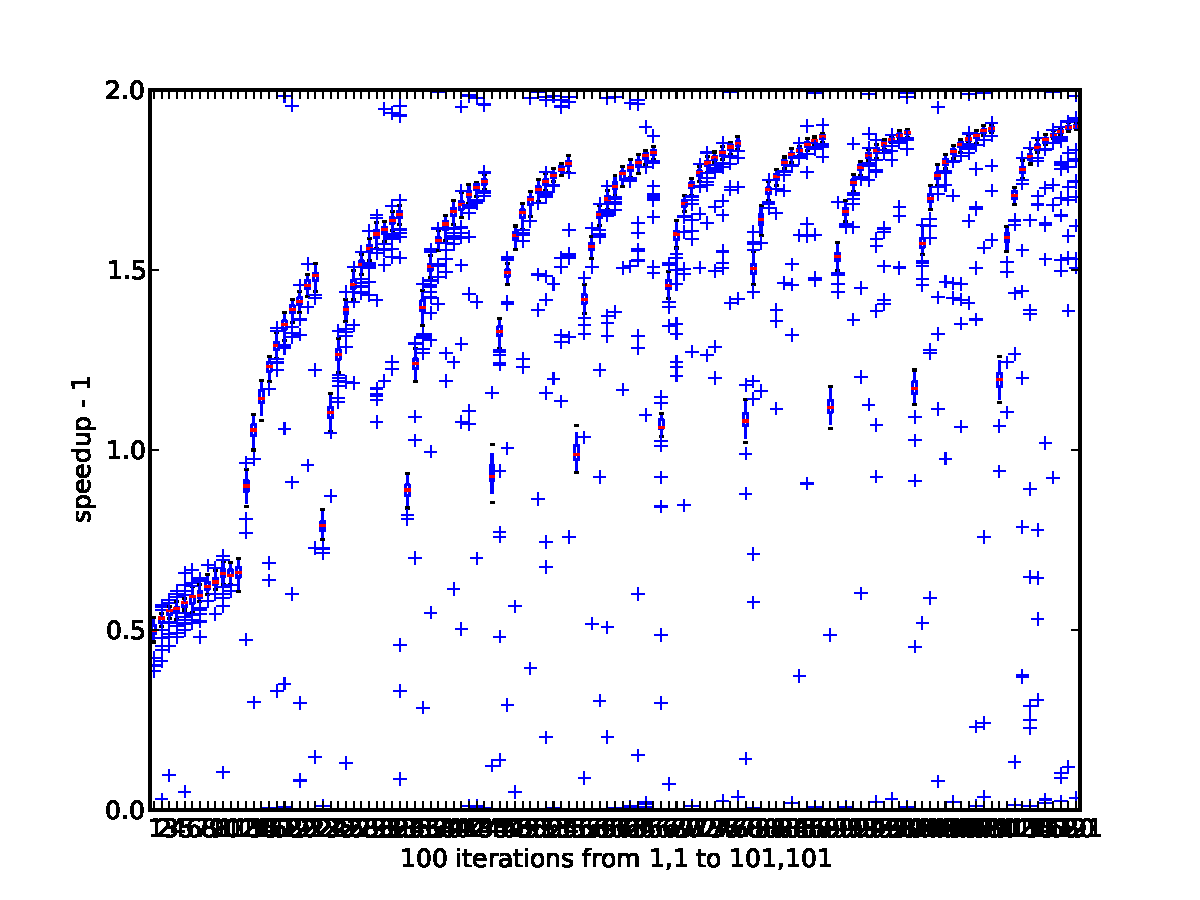
\includegraphics[scale=0.25]{images/openmp_measures_for_2_cores_n1_no_vartime_1_speedup_p1_pS10_P101_d1_dS10_D101_r100_s1.pdf}}
\subfloat[dynamicité sur 2 coeurs]{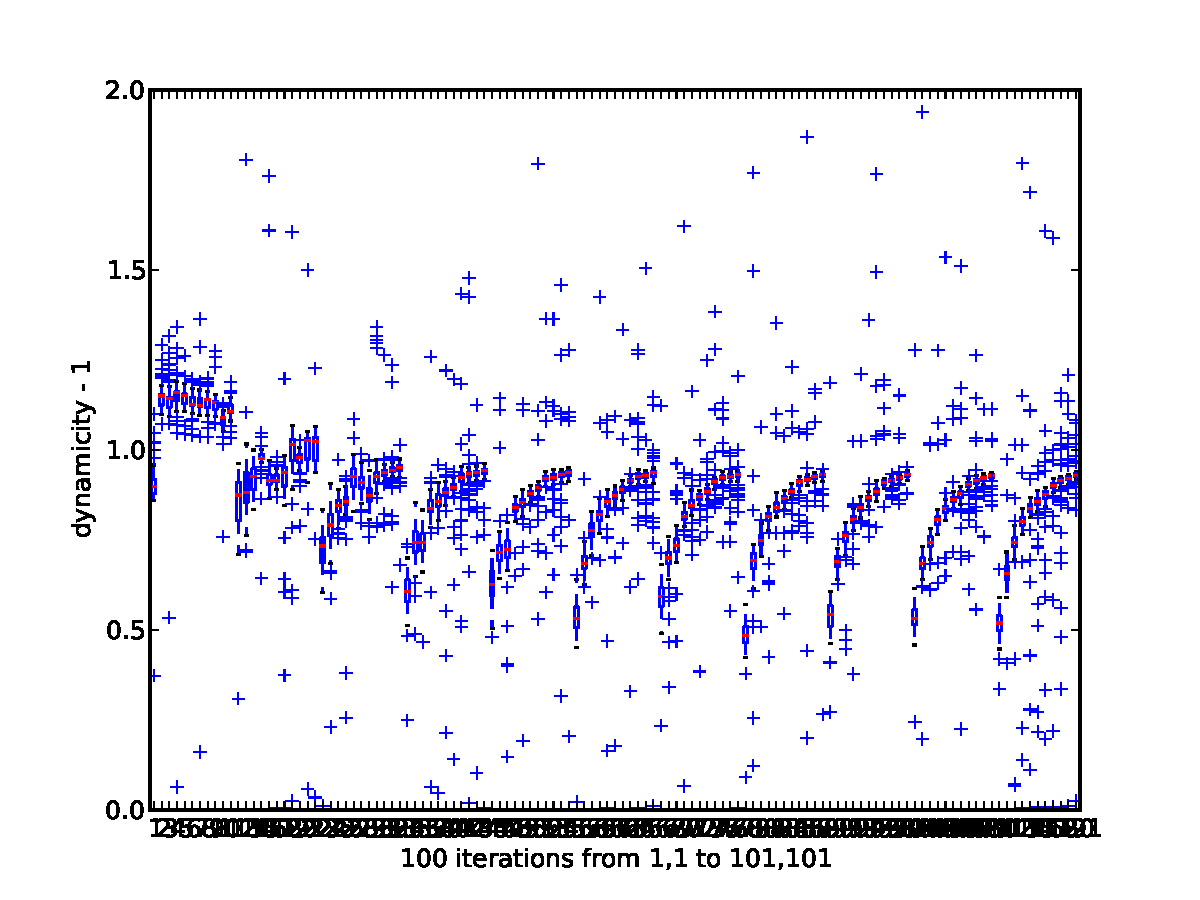
\includegraphics[scale=0.25]{images/openmp_measures_for_2_cores_n1_no_vartime_1_dynamicity_p1_pS10_P101_d1_dS10_D101_r100_s1.pdf}}
\qquad
\subfloat[speedup sur 8 coeurs]{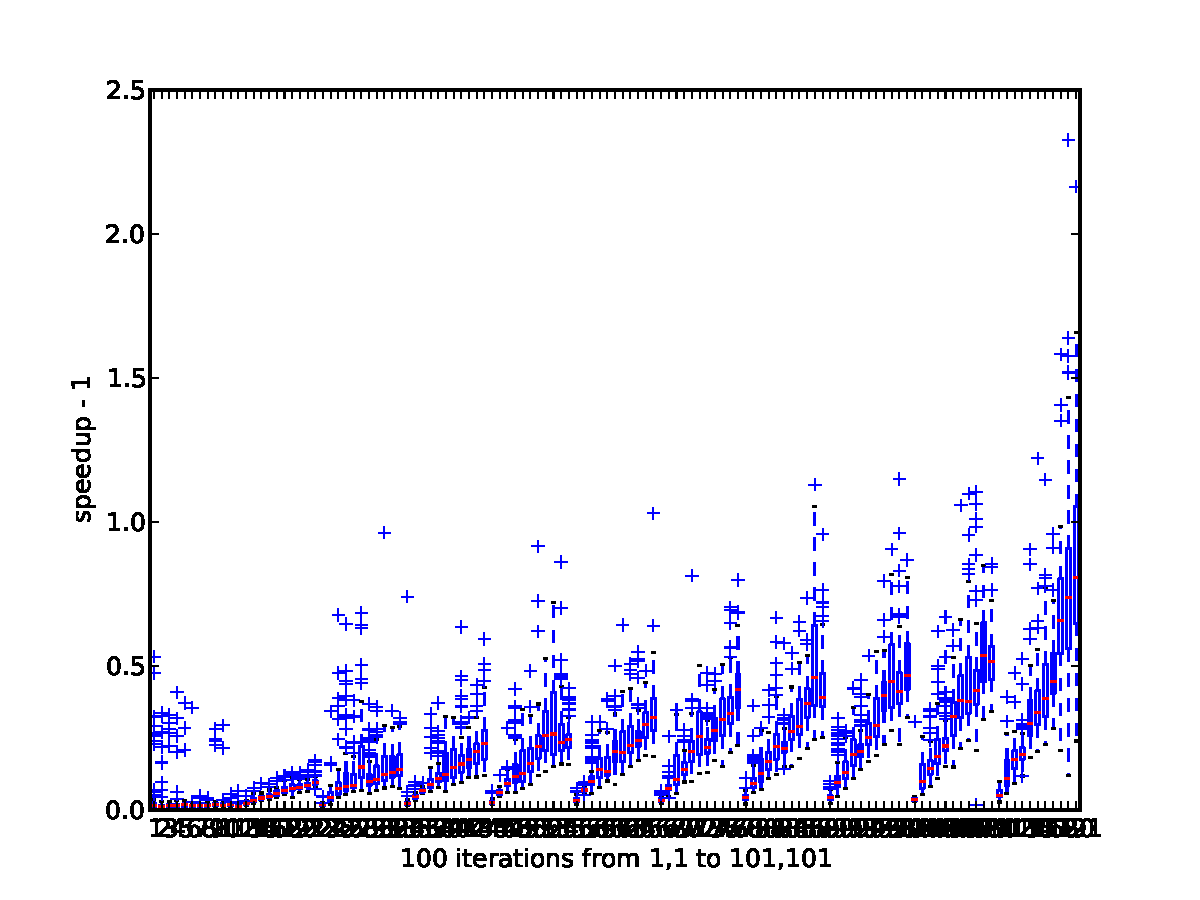
\includegraphics[scale=0.25]{images/openmp_measures_for_8_cores_n1_no_vartime_1_speedup_p1_pS10_P101_d1_dS10_D101_r100_s1.pdf}}
\subfloat[dynamicité sur 8 coeurs]{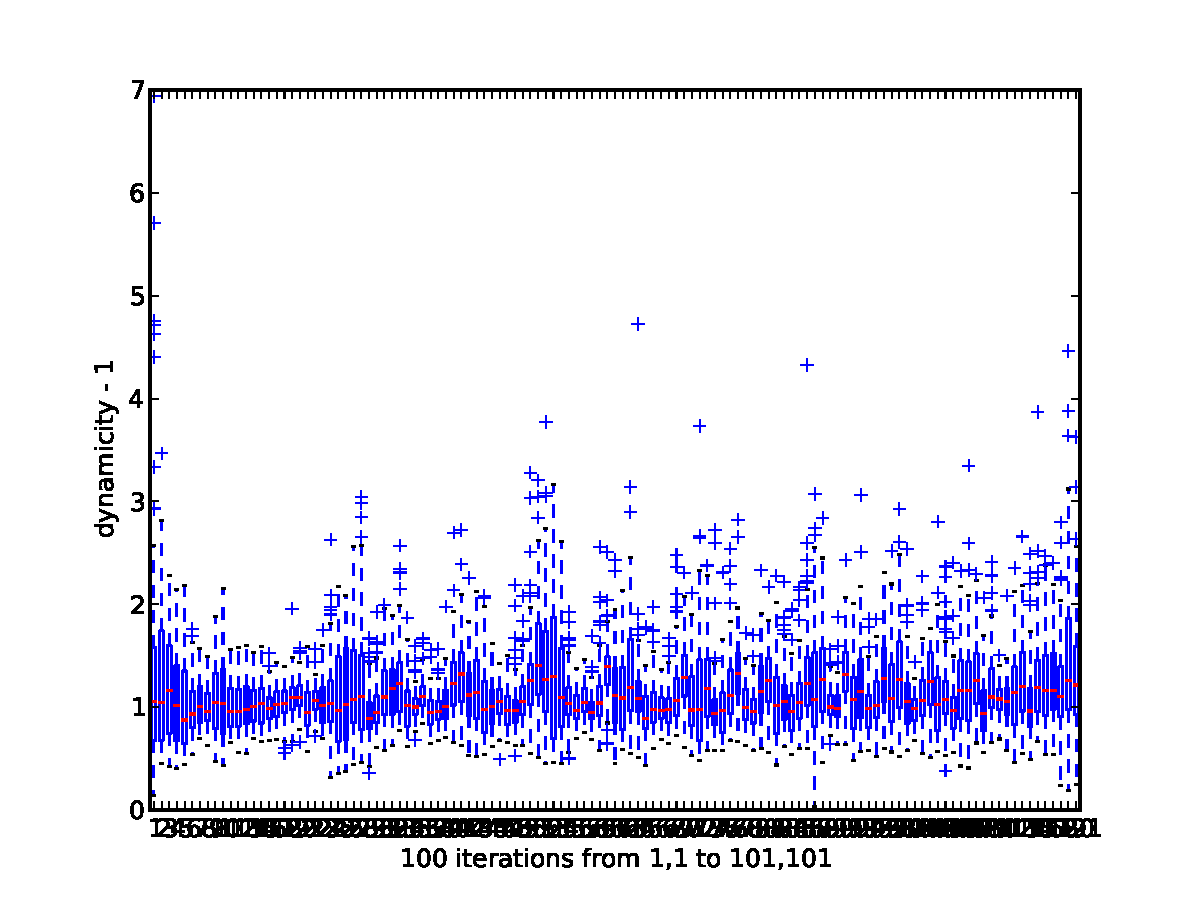
\includegraphics[scale=0.25]{images/openmp_measures_for_8_cores_n1_no_vartime_1_dynamicity_p1_pS10_P101_d1_dS10_D101_r100_s1.pdf}}
\caption{Mesure 1 en $O(1)$ sur 2 et 8 coeurs}
\label{fig:mesure_1_constant}
\end{figure}

% mesure 2 en O(1)
\begin{figure}[here]
\centering
\subfloat[speedup sur 2 coeurs]{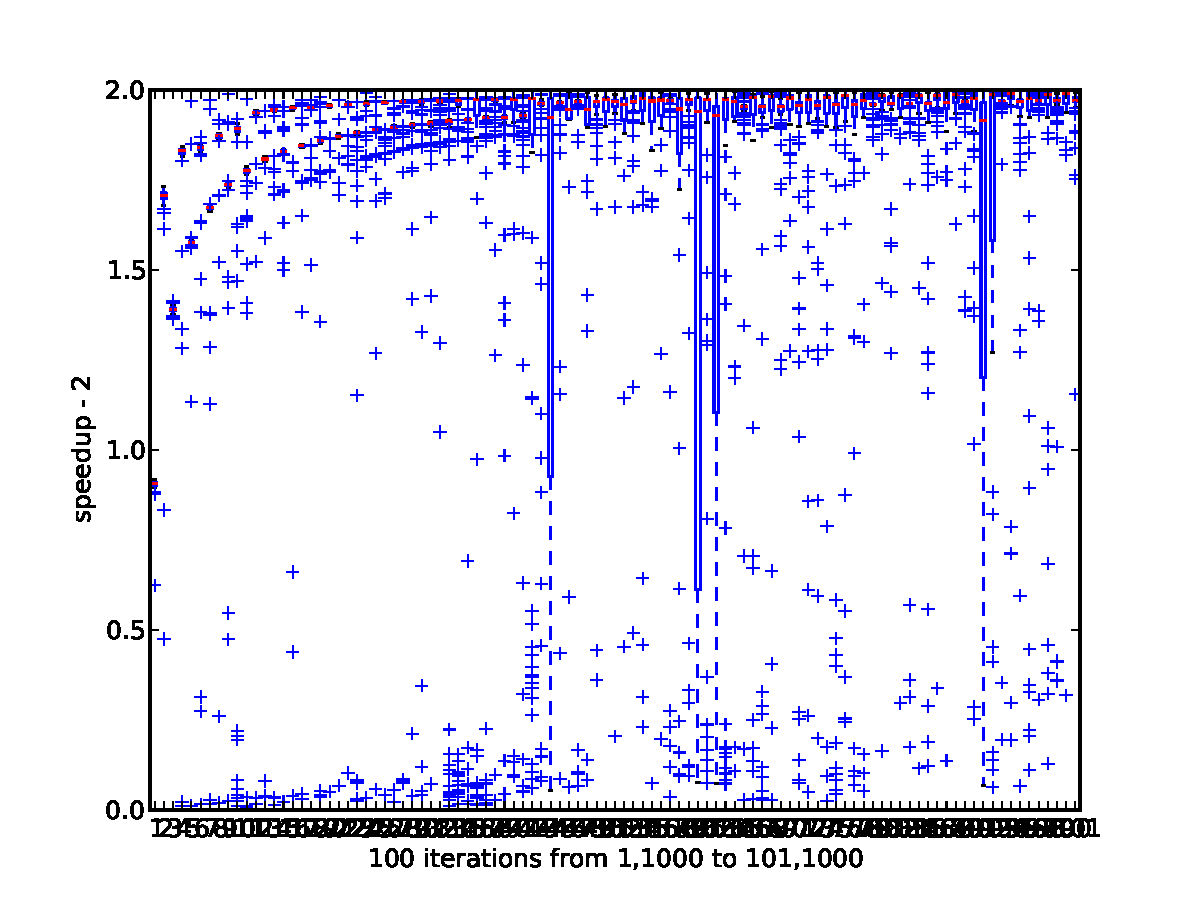
\includegraphics[scale=0.25]{images/openmp_measures_for_2_cores_n1_no_vartime_2_speedup_p1_pS1_P101_d1000_dS1_D1000_r100_s1.pdf}}
\subfloat[dynamicité sur 2 coeurs]{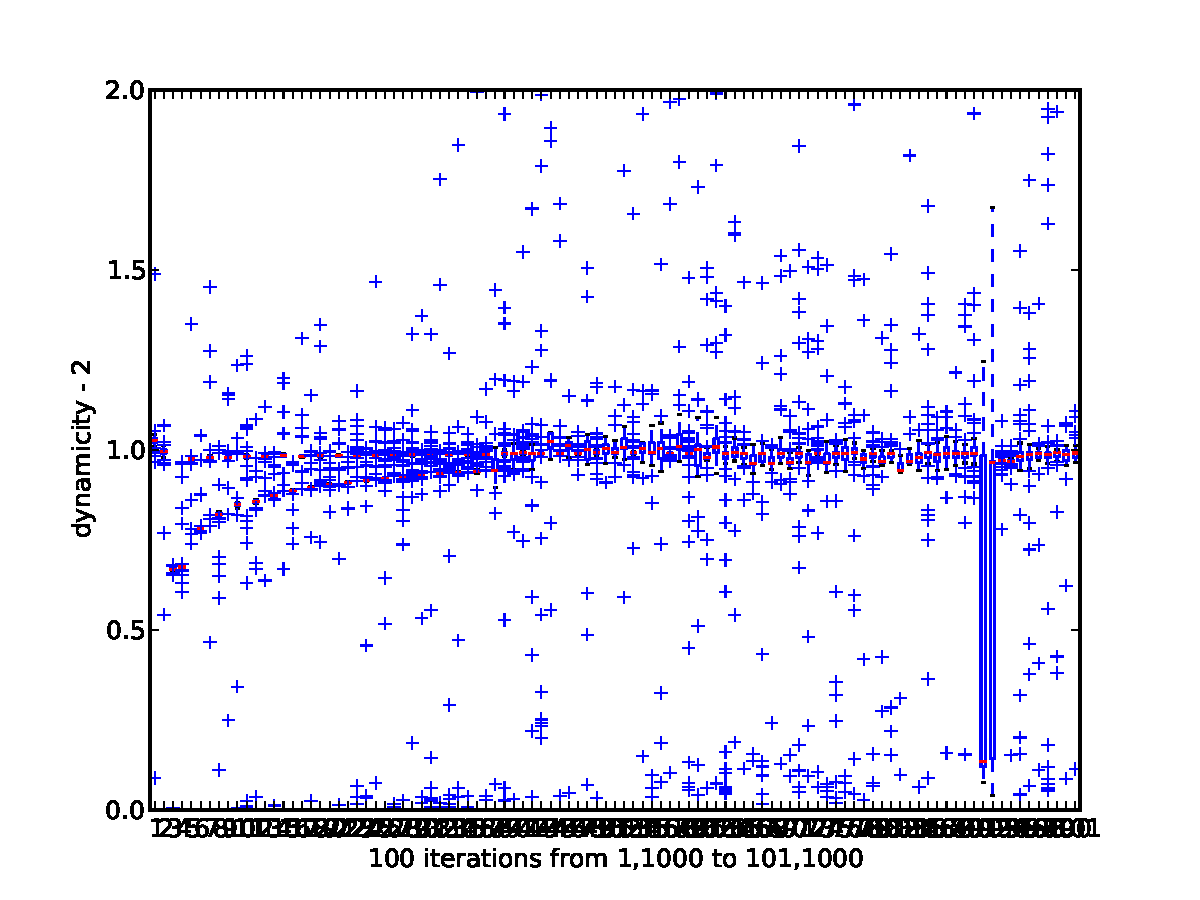
\includegraphics[scale=0.25]{images/openmp_measures_for_2_cores_n1_no_vartime_2_dynamicity_p1_pS1_P101_d1000_dS1_D1000_r100_s1.pdf}}
\qquad
\subfloat[speedup sur 8 coeurs]{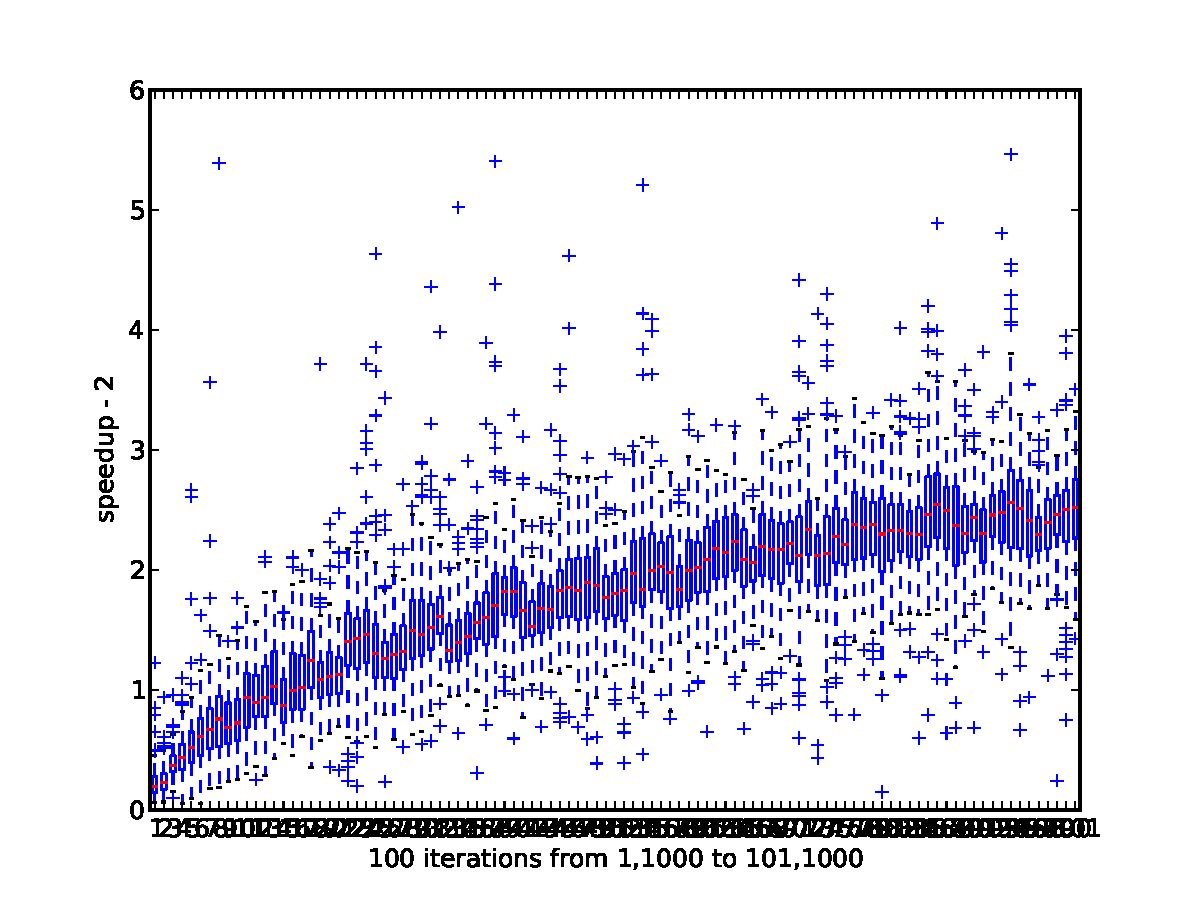
\includegraphics[scale=0.25]{images/openmp_measures_for_8_cores_n1_no_vartime_2_speedup_p1_pS1_P101_d1000_dS1_D1000_r100_s1.pdf}}
\subfloat[dynamicité sur 8 coeurs]{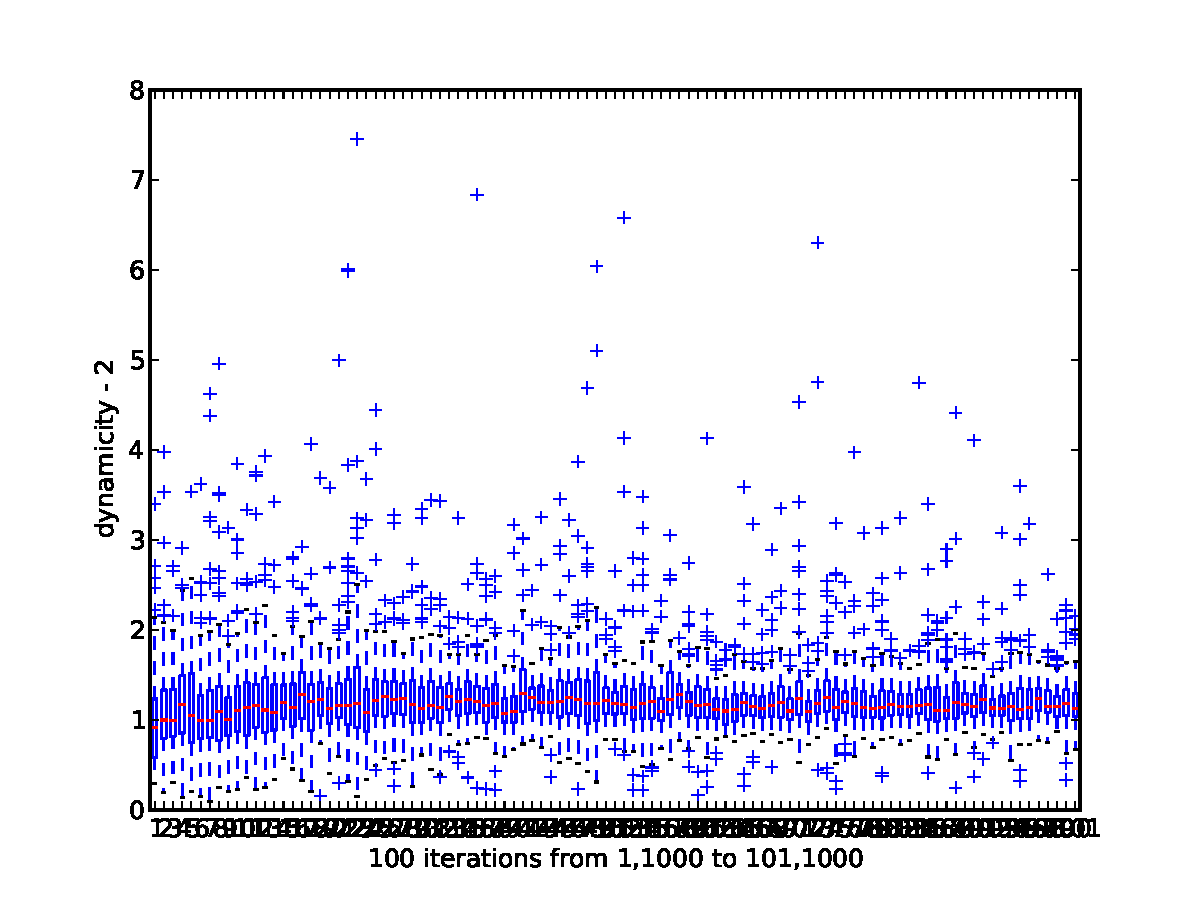
\includegraphics[scale=0.25]{images/openmp_measures_for_8_cores_n1_no_vartime_2_dynamicity_p1_pS1_P101_d1000_dS1_D1000_r100_s1.pdf}}
\caption{Mesure 2 en $O(1)$ sur 2 et 8 coeurs}
\label{fig:mesure_2_constant}
\end{figure}

% mesure 3 en O(1)
\begin{figure}[here]
\centering
\subfloat[speedup sur 2 coeurs]{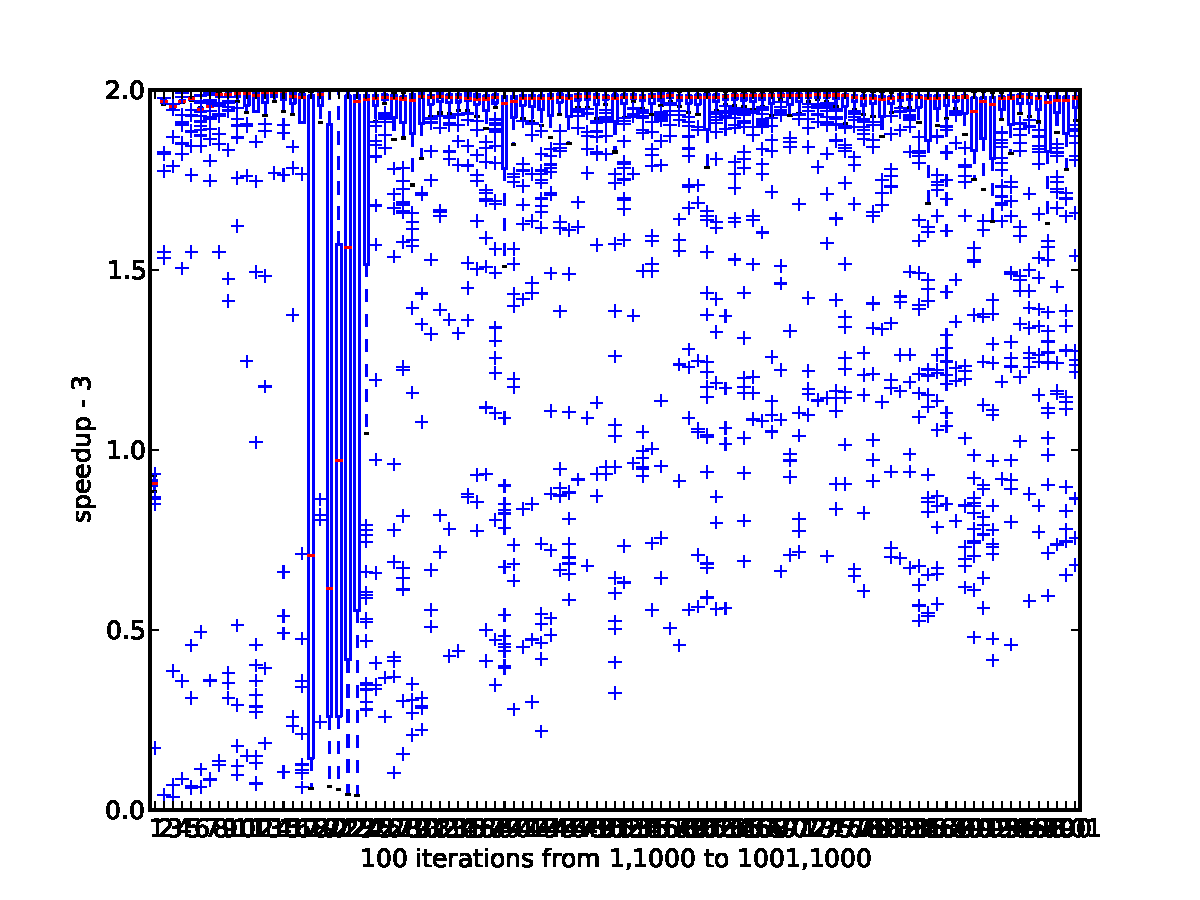
\includegraphics[scale=0.25]{images/openmp_measures_for_2_cores_n1_no_vartime_3_speedup_p1_pS10_P1001_d1000_dS1_D1000_r100_s1.pdf}}
\subfloat[dynamicité sur 2 coeurs]{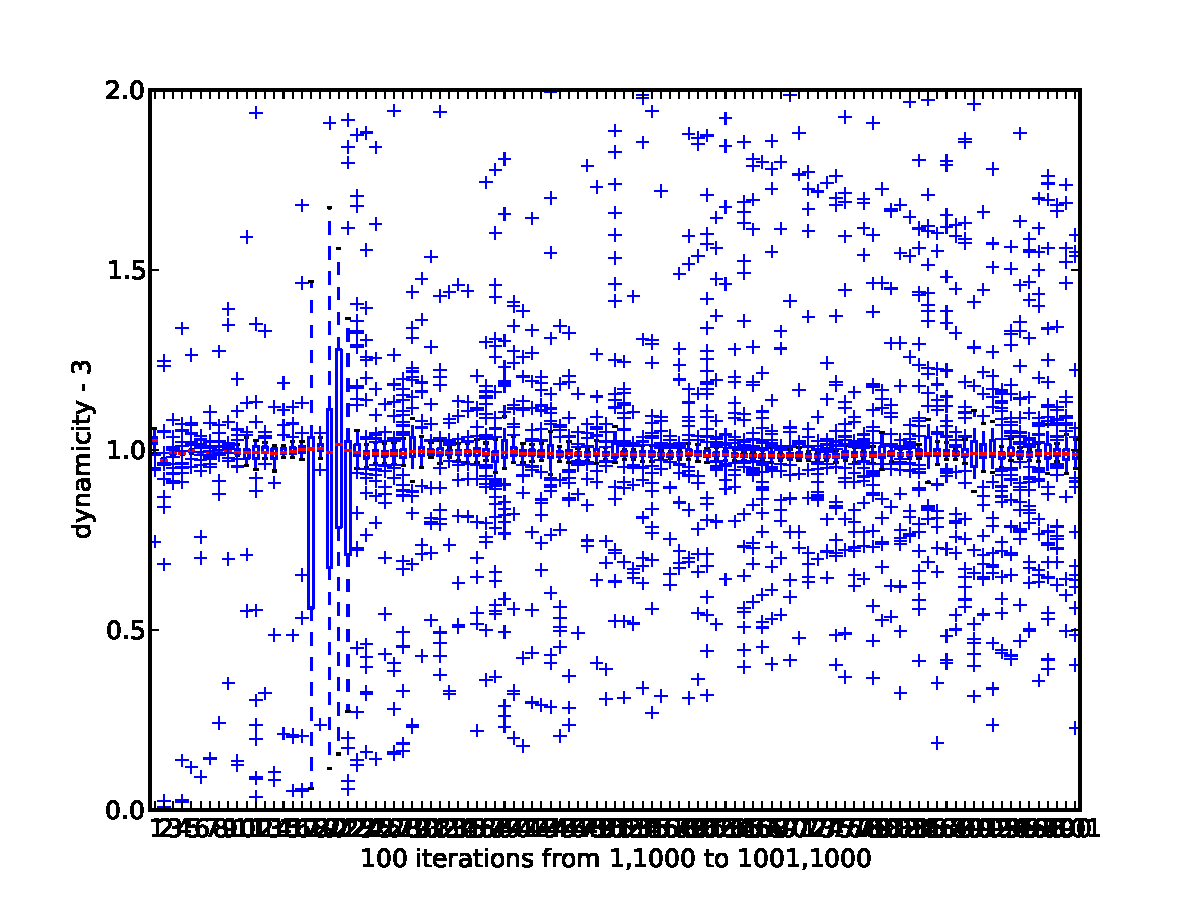
\includegraphics[scale=0.25]{images/openmp_measures_for_2_cores_n1_no_vartime_3_dynamicity_p1_pS10_P1001_d1000_dS1_D1000_r100_s1.pdf}}
\qquad
\subfloat[speedup sur 8 coeurs]{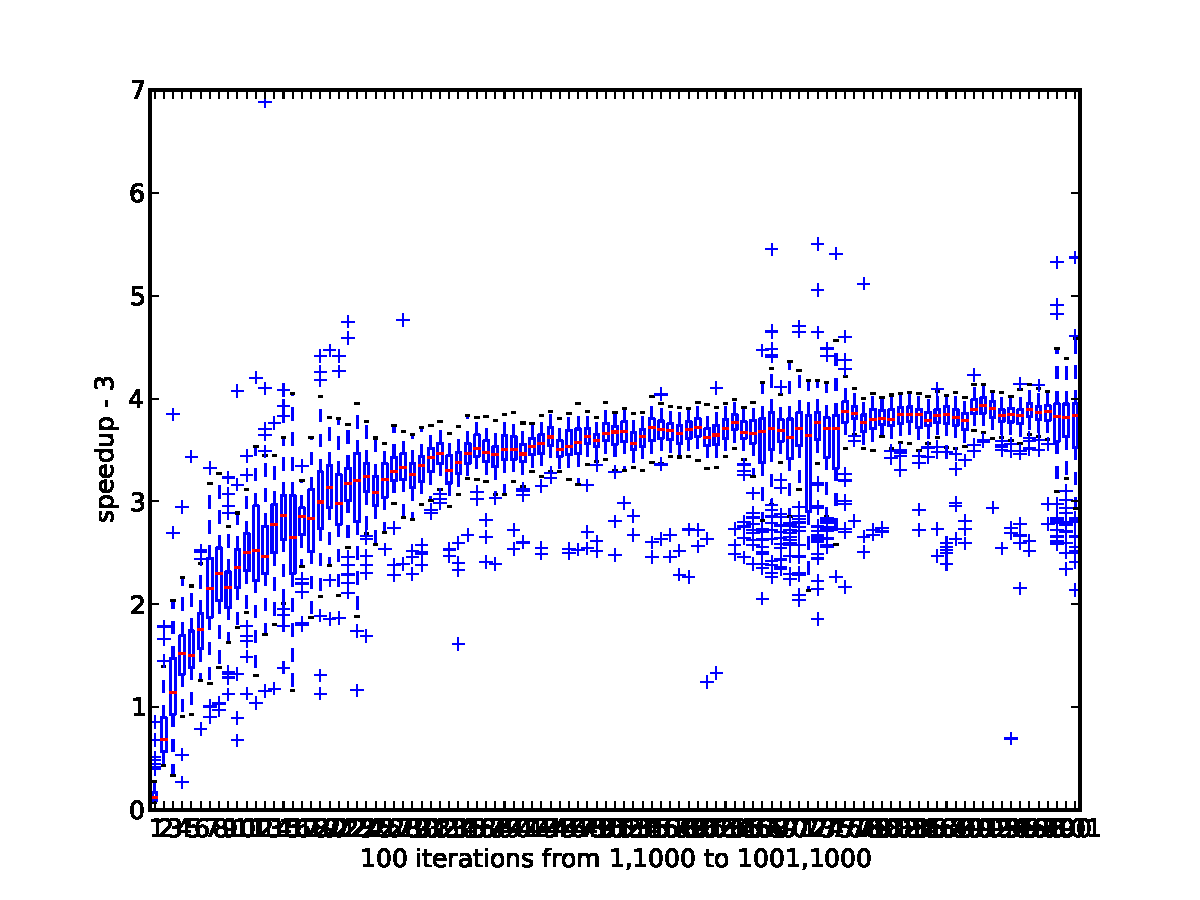
\includegraphics[scale=0.25]{images/openmp_measures_for_8_cores_n1_no_vartime_3_speedup_p1_pS10_P1001_d1000_dS1_D1000_r100_s1.pdf}}
\subfloat[dynamicité sur 8 coeurs]{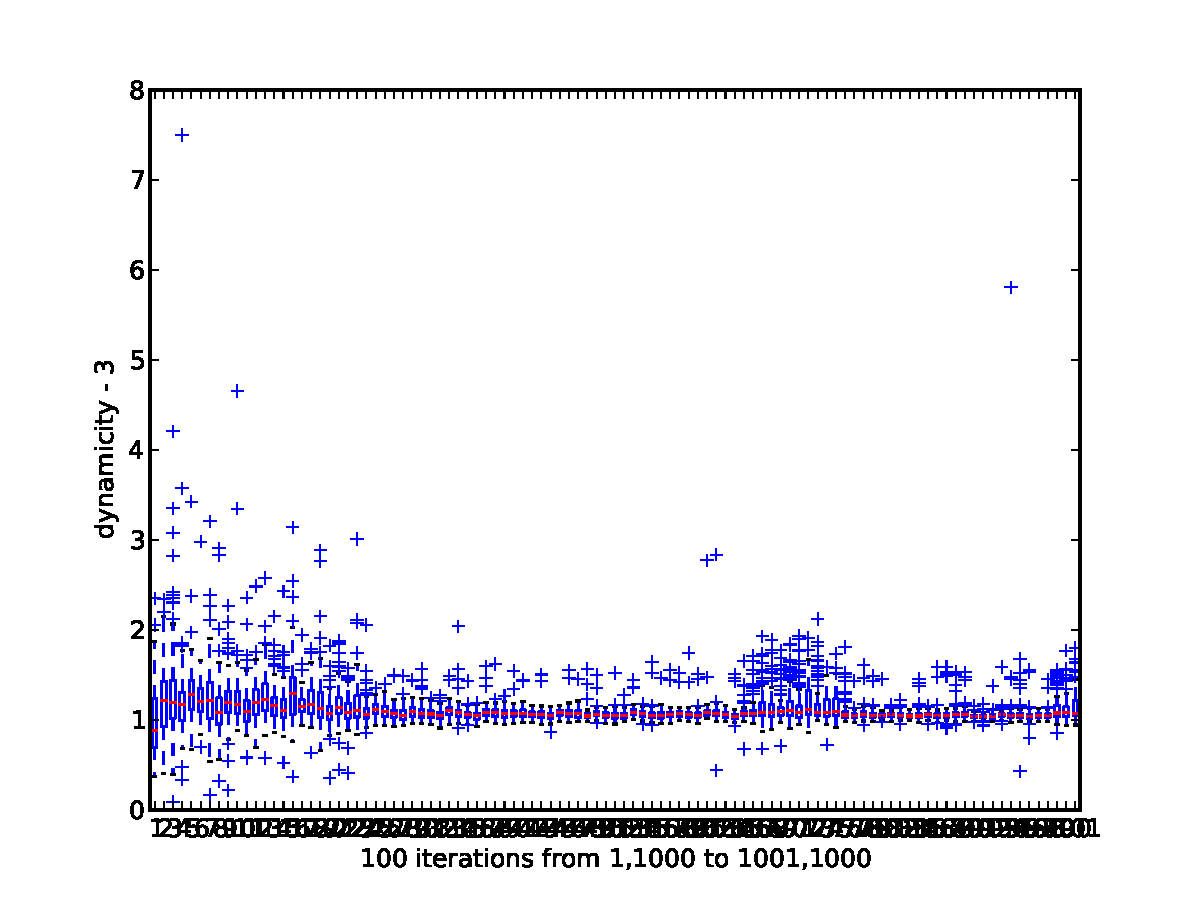
\includegraphics[scale=0.25]{images/openmp_measures_for_8_cores_n1_no_vartime_3_dynamicity_p1_pS10_P1001_d1000_dS1_D1000_r100_s1.pdf}}
\caption{Mesure 3 en $O(1)$ sur 2 et 8 coeurs}
\label{fig:mesure_3_constant}
\end{figure}

% mesure 4 en O(1)
\begin{figure}[here]
\centering
\subfloat[speedup sur 2 coeurs]{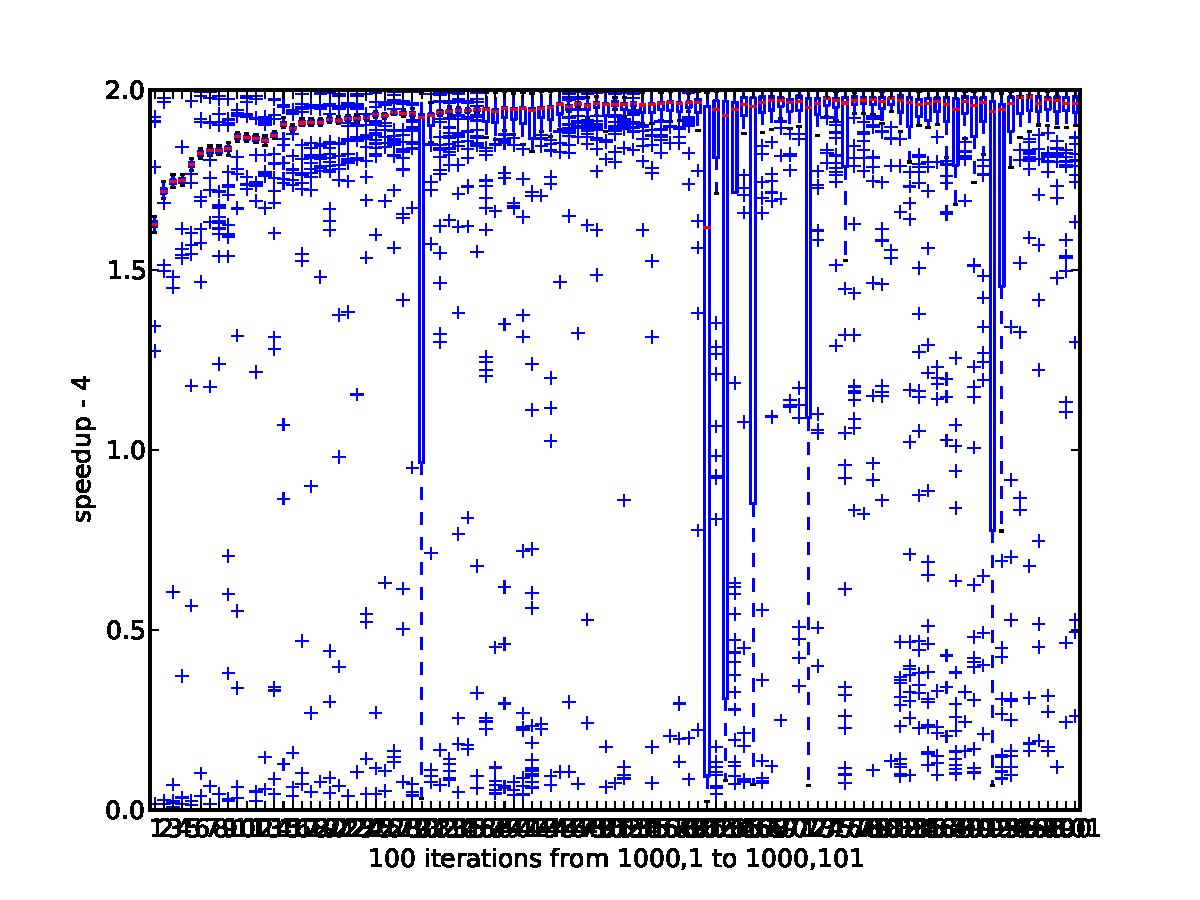
\includegraphics[scale=0.25]{images/openmp_measures_for_2_cores_n1_no_vartime_4_speedup_p1000_pS1_P1000_d1_dS1_D101_r100_s1.pdf}}
\subfloat[dynamicité sur 2 coeurs]{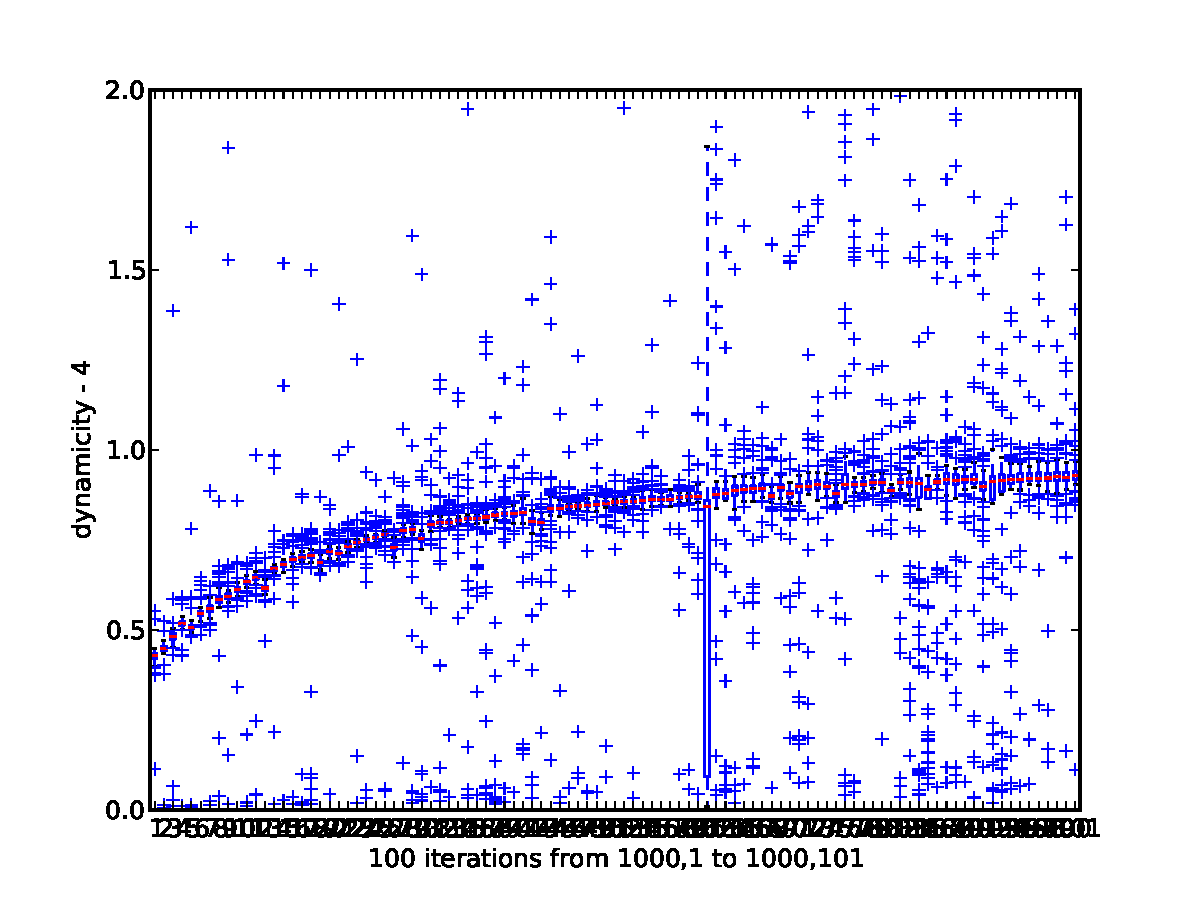
\includegraphics[scale=0.25]{images/openmp_measures_for_2_cores_n1_no_vartime_4_dynamicity_p1000_pS1_P1000_d1_dS1_D101_r100_s1.pdf}}
\qquad
\subfloat[speedup sur 8 coeurs]{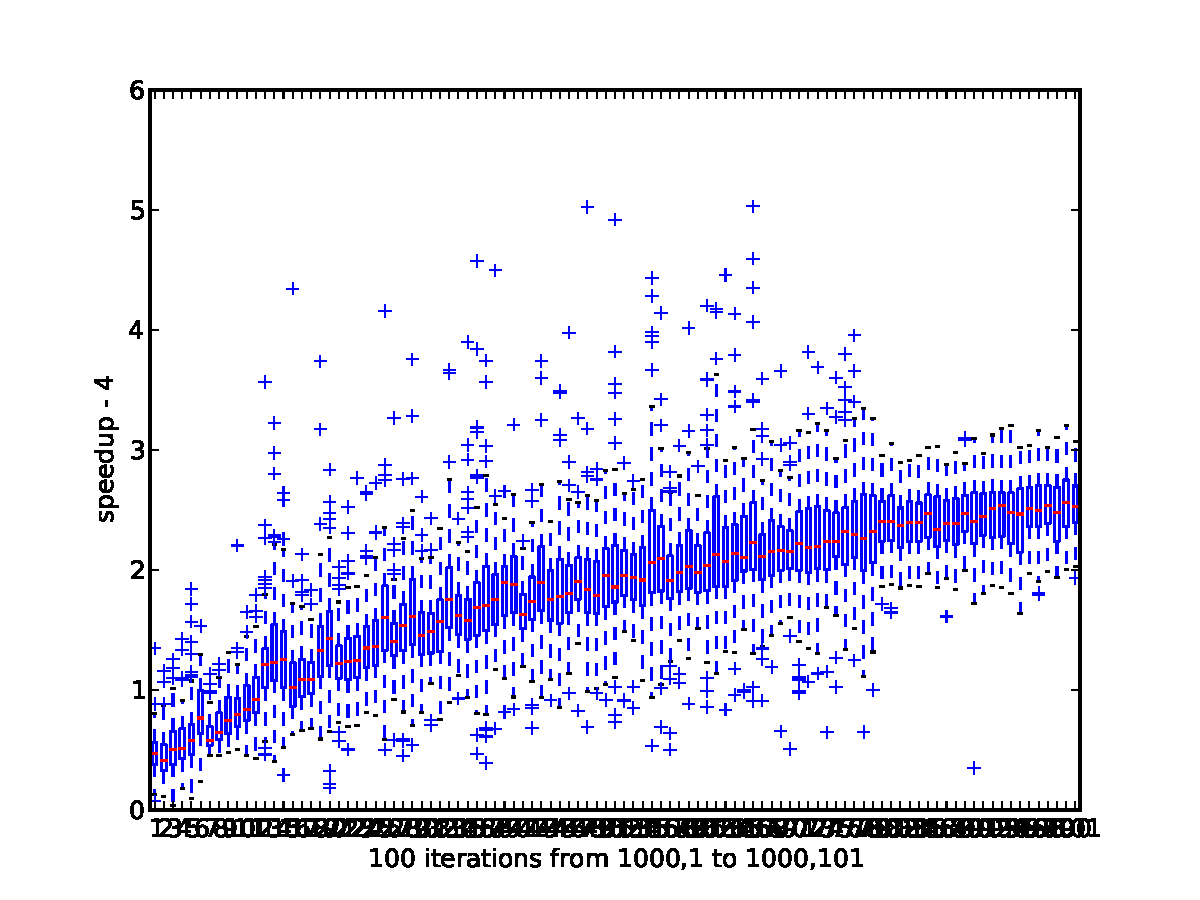
\includegraphics[scale=0.25]{images/openmp_measures_for_8_cores_n1_no_vartime_4_speedup_p1000_pS1_P1000_d1_dS1_D101_r100_s1.pdf}}
\subfloat[dynamicité sur 8 coeurs]{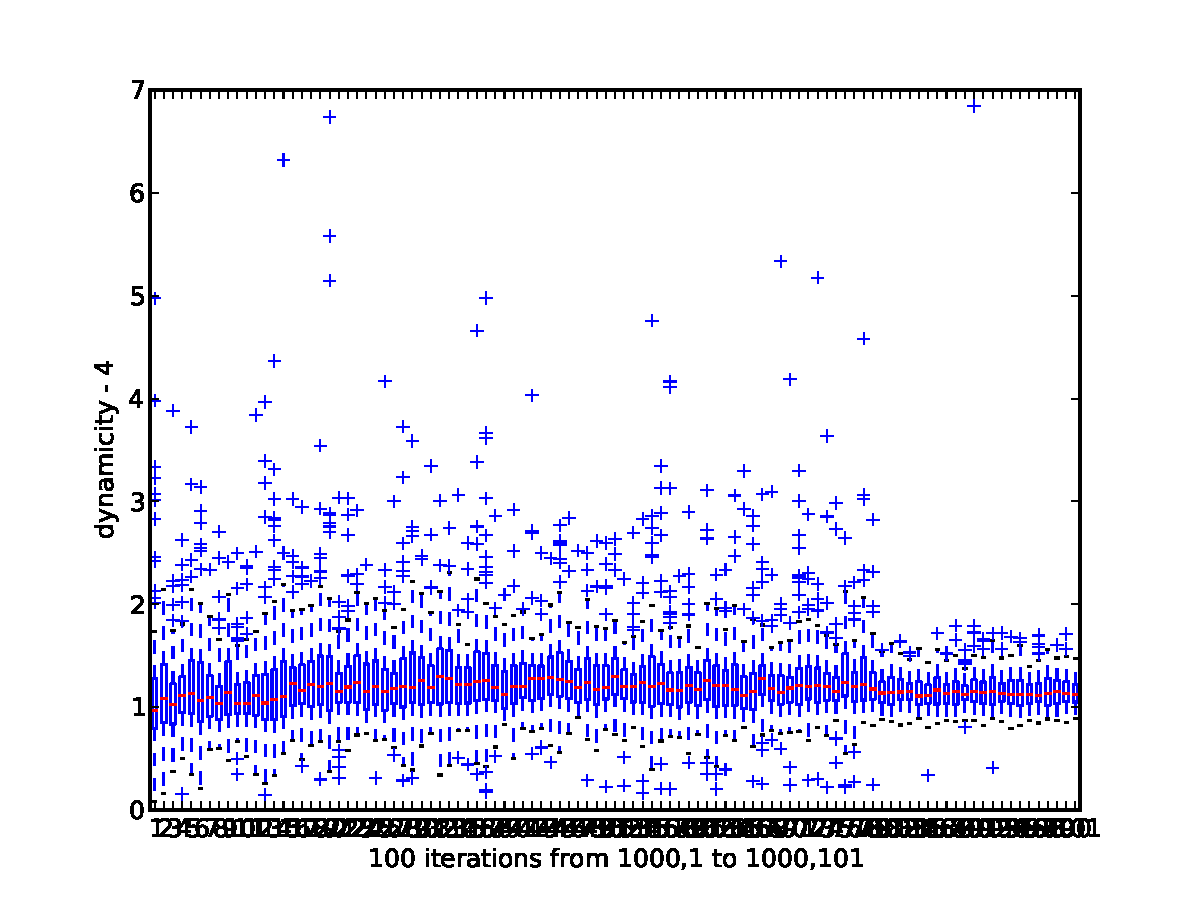
\includegraphics[scale=0.25]{images/openmp_measures_for_8_cores_n1_no_vartime_4_dynamicity_p1000_pS1_P1000_d1_dS1_D101_r100_s1.pdf}}
\caption{Mesure 4 en $O(1)$ sur 2 et 8 coeurs}
\label{fig:mesure_4_constant}
\end{figure}

% mesure 5 en O(1)
\begin{figure}[here]
\centering
\subfloat[speedup sur 2 coeurs]{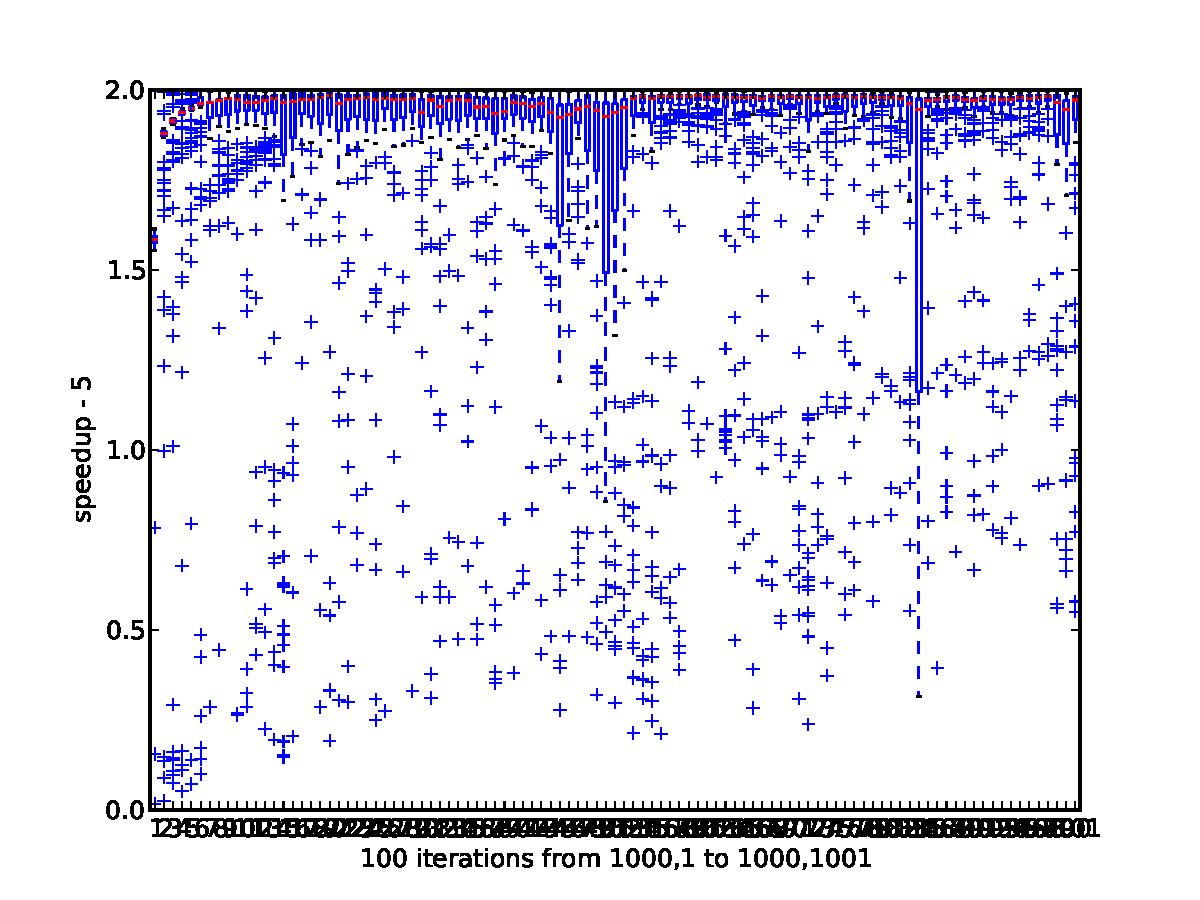
\includegraphics[scale=0.25]{images/openmp_measures_for_2_cores_n1_no_vartime_5_speedup_p1000_pS1_P1000_d1_dS10_D1001_r100_s1.pdf}}
\subfloat[dynamicité sur 2 coeurs]{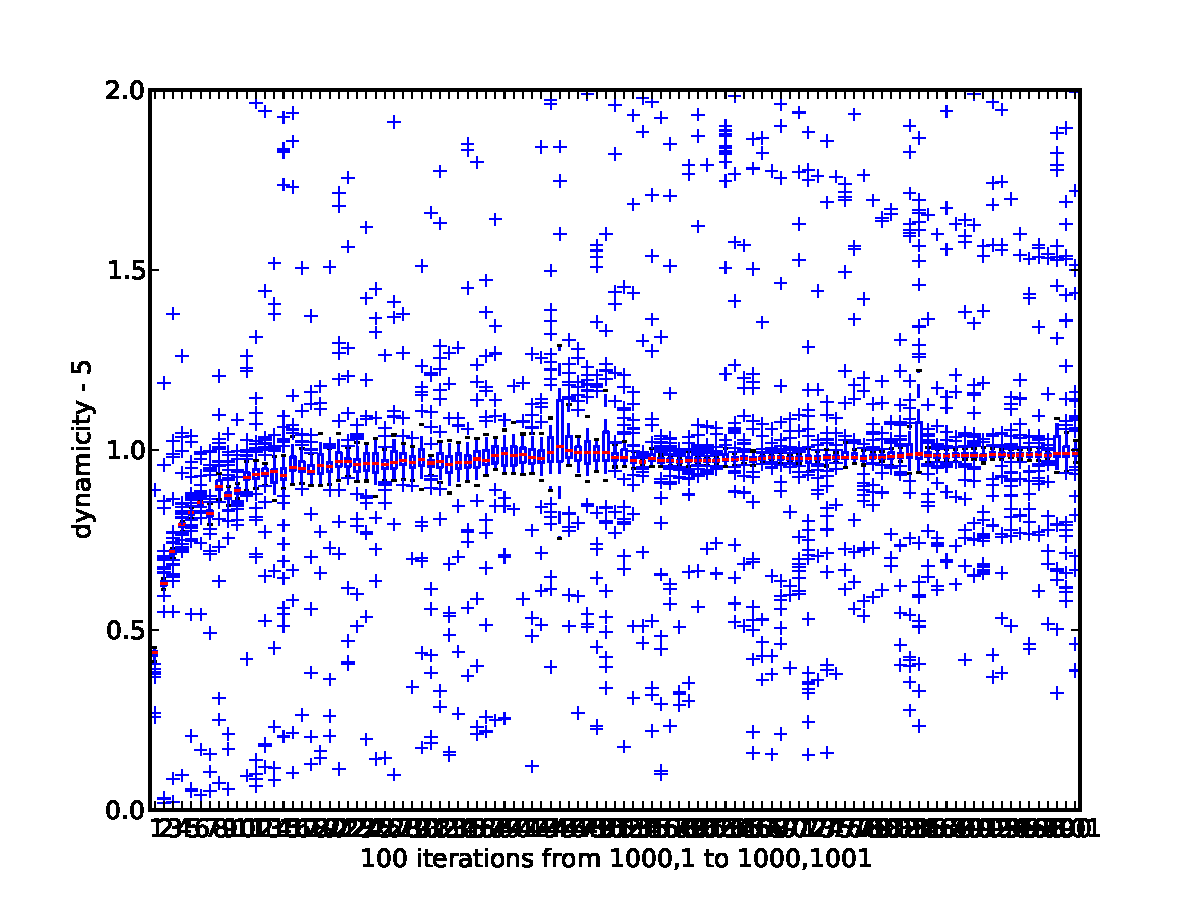
\includegraphics[scale=0.25]{images/openmp_measures_for_2_cores_n1_no_vartime_5_dynamicity_p1000_pS1_P1000_d1_dS10_D1001_r100_s1.pdf}}
\qquad
\subfloat[speedup sur 8 coeurs]{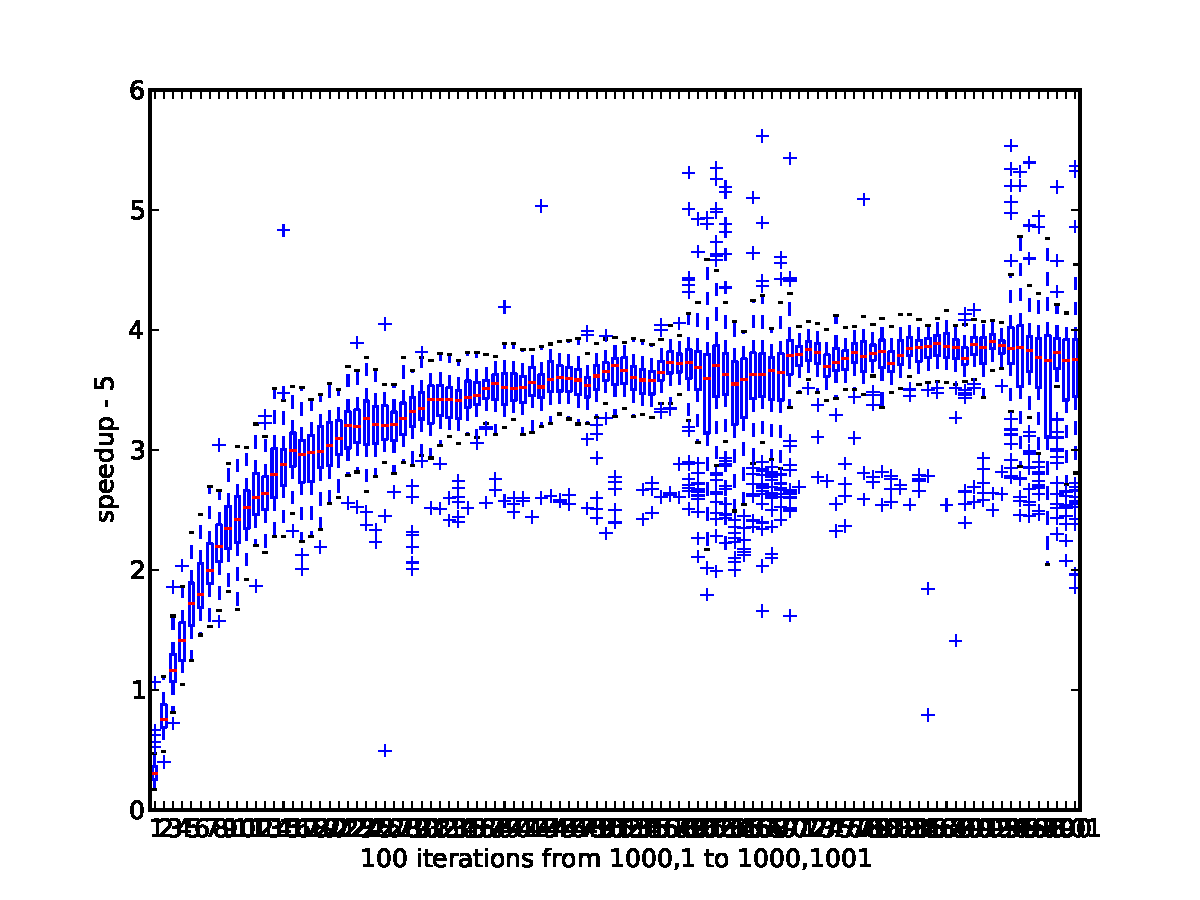
\includegraphics[scale=0.25]{images/openmp_measures_for_8_cores_n1_no_vartime_5_speedup_p1000_pS1_P1000_d1_dS10_D1001_r100_s1.pdf}}
\subfloat[dynamicité sur 8 coeurs]{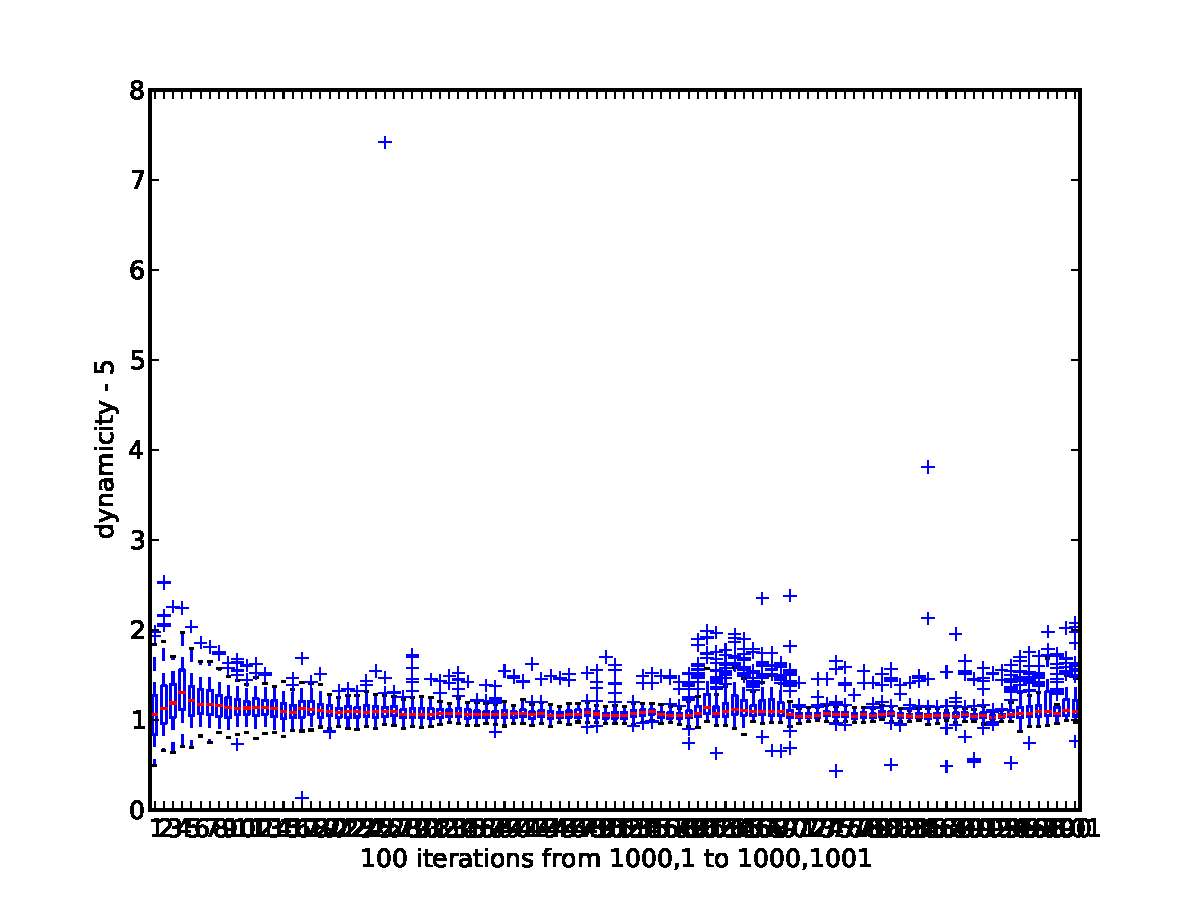
\includegraphics[scale=0.25]{images/openmp_measures_for_8_cores_n1_no_vartime_5_dynamicity_p1000_pS1_P1000_d1_dS10_D1001_r100_s1.pdf}}
\caption{Mesure 5 en $O(1)$ sur 2 et 8 coeurs}
\label{fig:mesure_5_constant}
\end{figure}

\newpage

\subsubsection{Résultats en $O(n)$}

Dans un second temps, le benchmark est exécuté pour le problème qui se résoud en temps variable. Les résultats de chaque mesure sont numérotés d'après le tableau des mesures décrit précédemment en figure \ref{fig:liste_mesures}.\\

Il est important d'ajouter que compte tenu de la résolution du problème en $O(n)$ et non plus en fonction de la dimension, celle ci perd de son importance. Ainsi les mesures 1, 4 et 5 ne sont plus nessaire à mesurer. Seules les mesures 2 et 3 seront présentées ci-dessous.\\

Un algorithme séquentiel exécuté sur un processeur à 8 coeurs en comparaison avec un processeur à 2 coeurs est plus performant sur des petits échantillons. Nous avons donc choisit de définir les bornes des paramètres, décrits en figure \ref{fig:liste_mesures}, comme multiple du nombre de coeurs disponible.\\

Les mesures sont présentées en fonction des processeurs utilisés et disponibles en figure \ref{fig:mesure_2_variable} et \ref{fig:mesure_3_variable}.

% mesure 2 en O(n)
\begin{figure}[here]
\centering
\subfloat[speedup sur 2 coeurs]{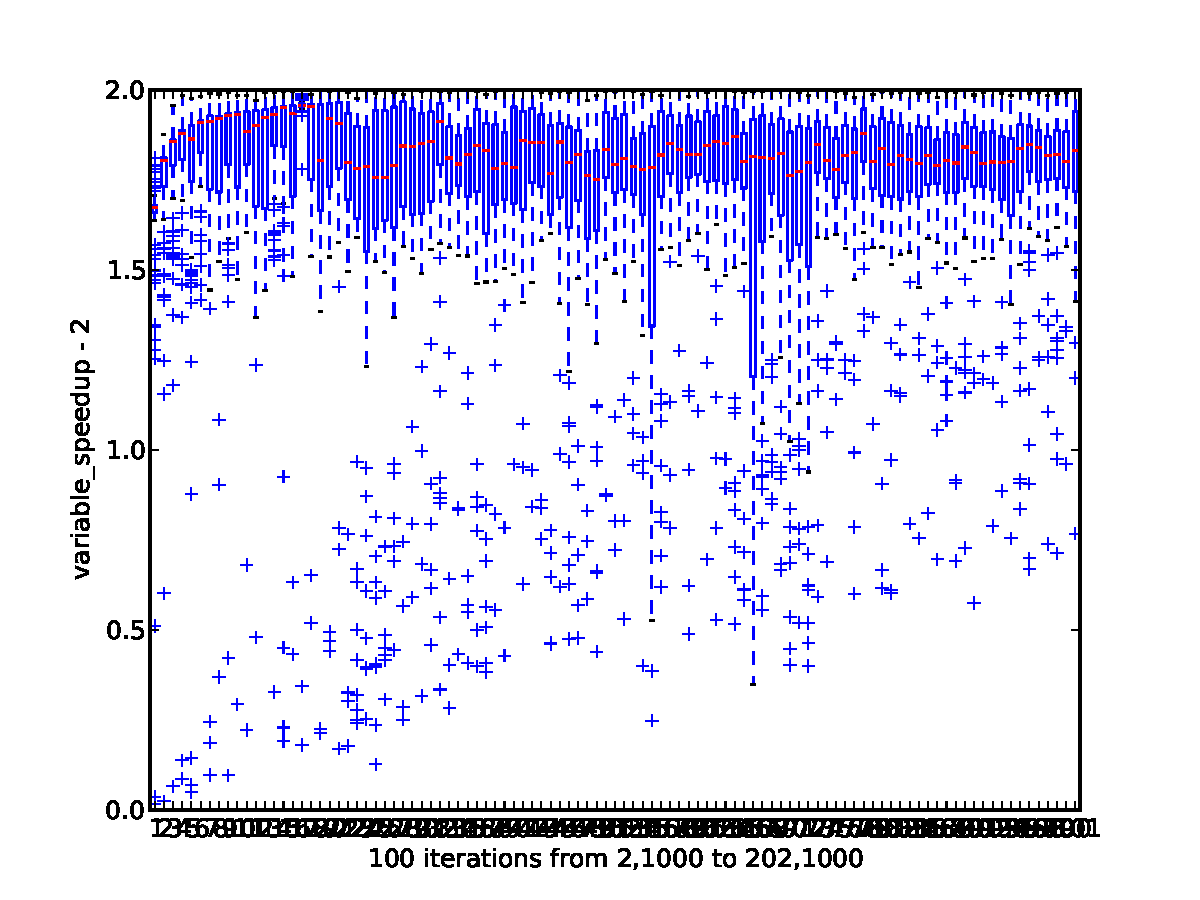
\includegraphics[scale=0.25]{images/openmp_measures_for_2_cores_n2_2_variable_speedup_p2_pS2_P202_d1000_dS1_D1000_r100_s1.pdf}}
\subfloat[dynamicité sur 2 coeurs]{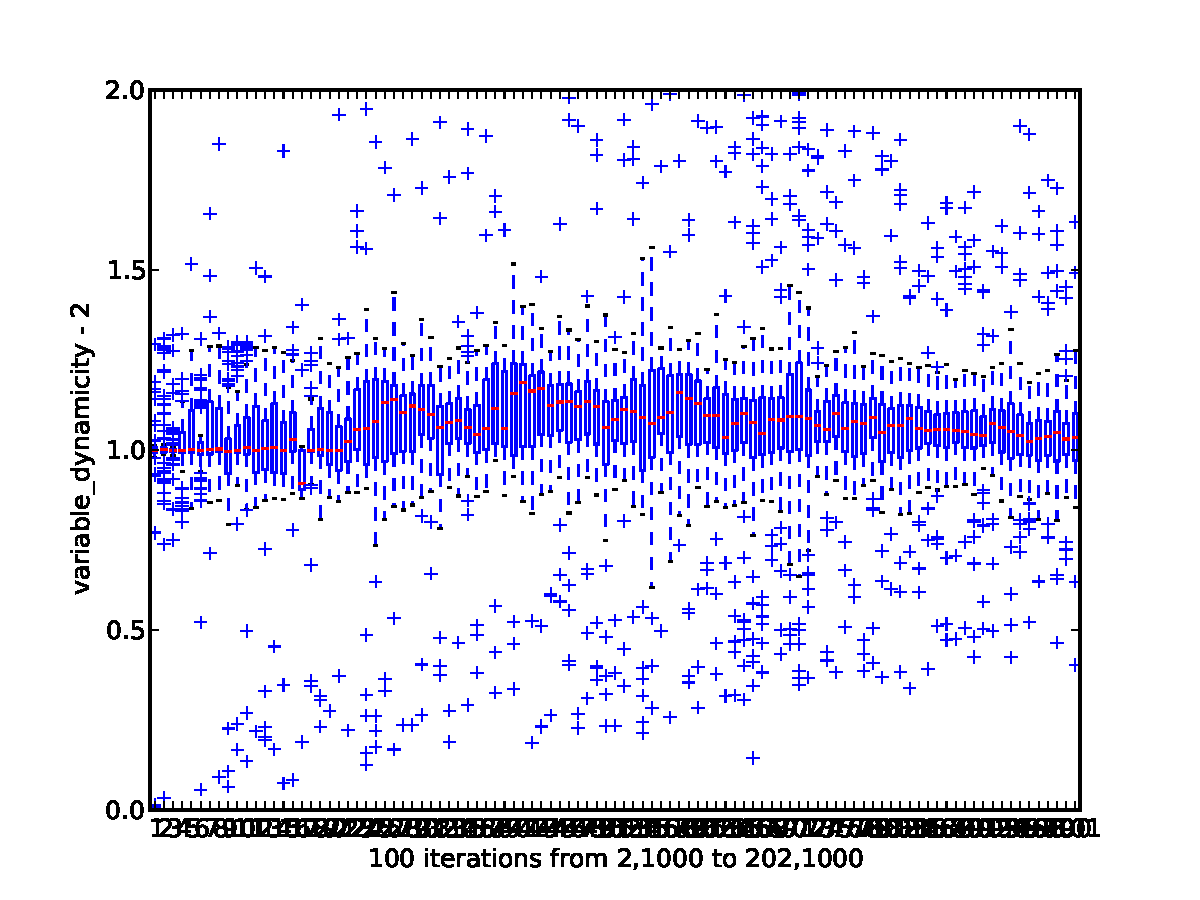
\includegraphics[scale=0.25]{images/openmp_measures_for_2_cores_n2_2_variable_dynamicity_p2_pS2_P202_d1000_dS1_D1000_r100_s1.pdf}}
\qquad
\subfloat[speedup sur 8 coeurs]{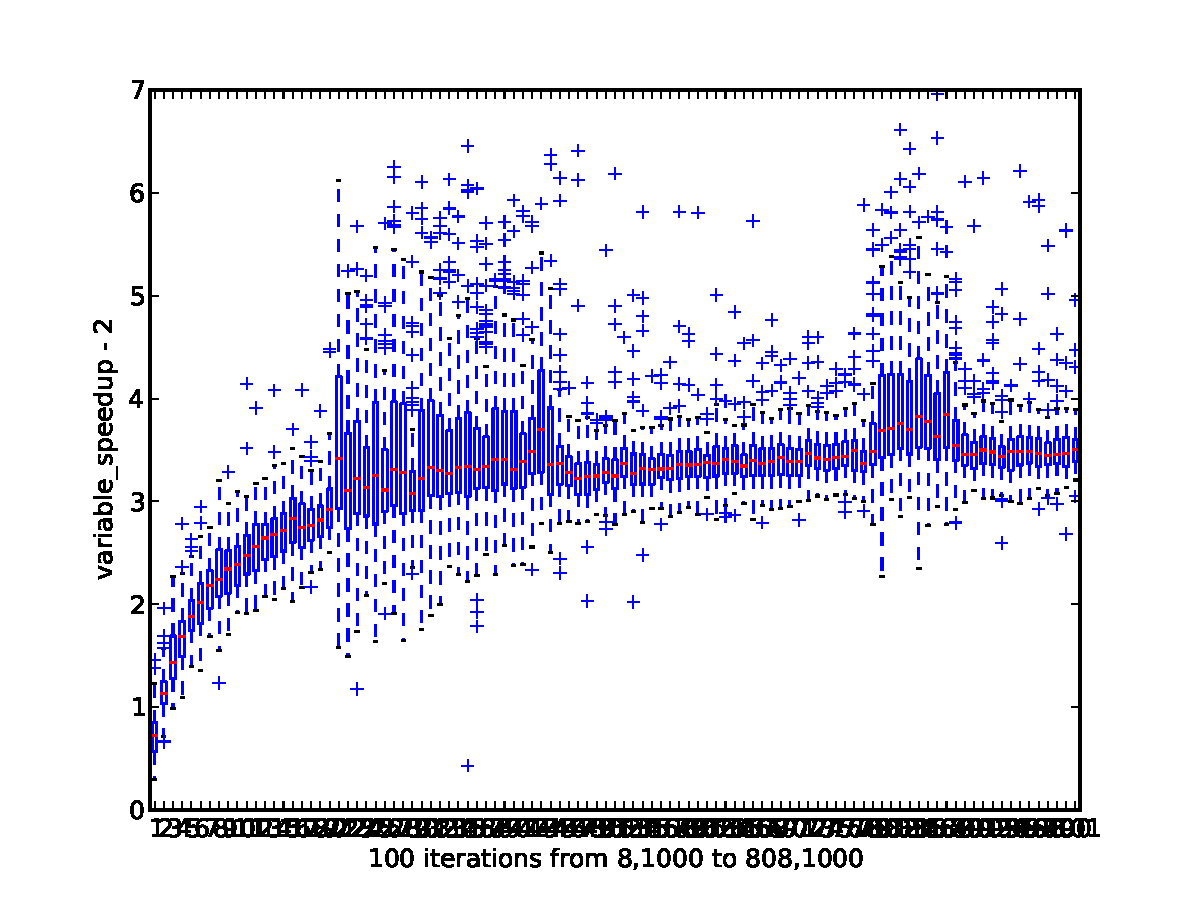
\includegraphics[scale=0.25]{images/openmp_measures_for_8_cores_n8_no_consttime_2_variable_speedup_p8_pS8_P808_d1000_dS1_D1000_r100_s1.pdf}}
\subfloat[dynamicité sur 8 coeurs]{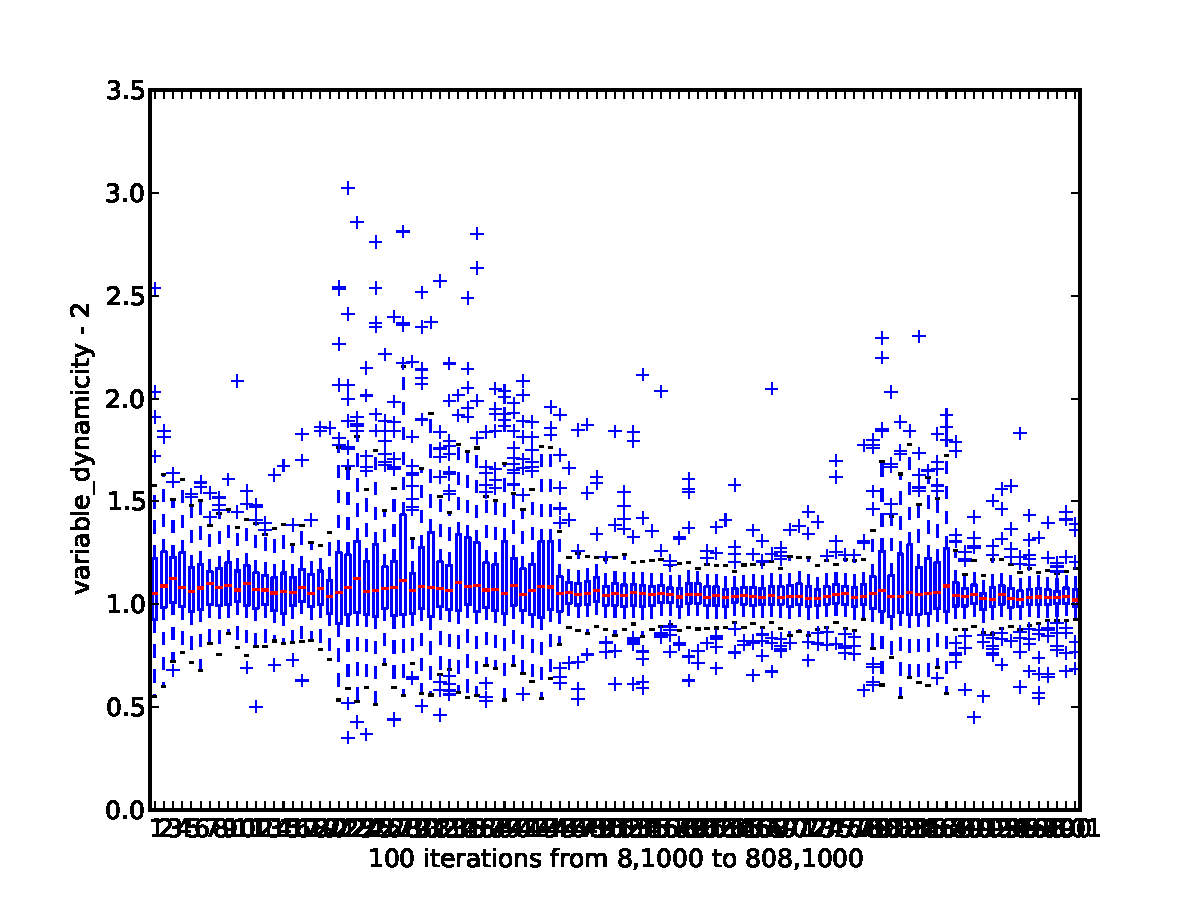
\includegraphics[scale=0.25]{images/openmp_measures_for_8_cores_n8_no_consttime_2_variable_dynamicity_p8_pS8_P808_d1000_dS1_D1000_r100_s1.pdf}}
\caption{Mesure 2 en $O(n)$ sur 2 et 8 coeurs}
\label{fig:mesure_2_variable}
\end{figure}

% mesure 3 en O(1)
\begin{figure}[here]
\centering
\subfloat[speedup sur 2 coeurs]{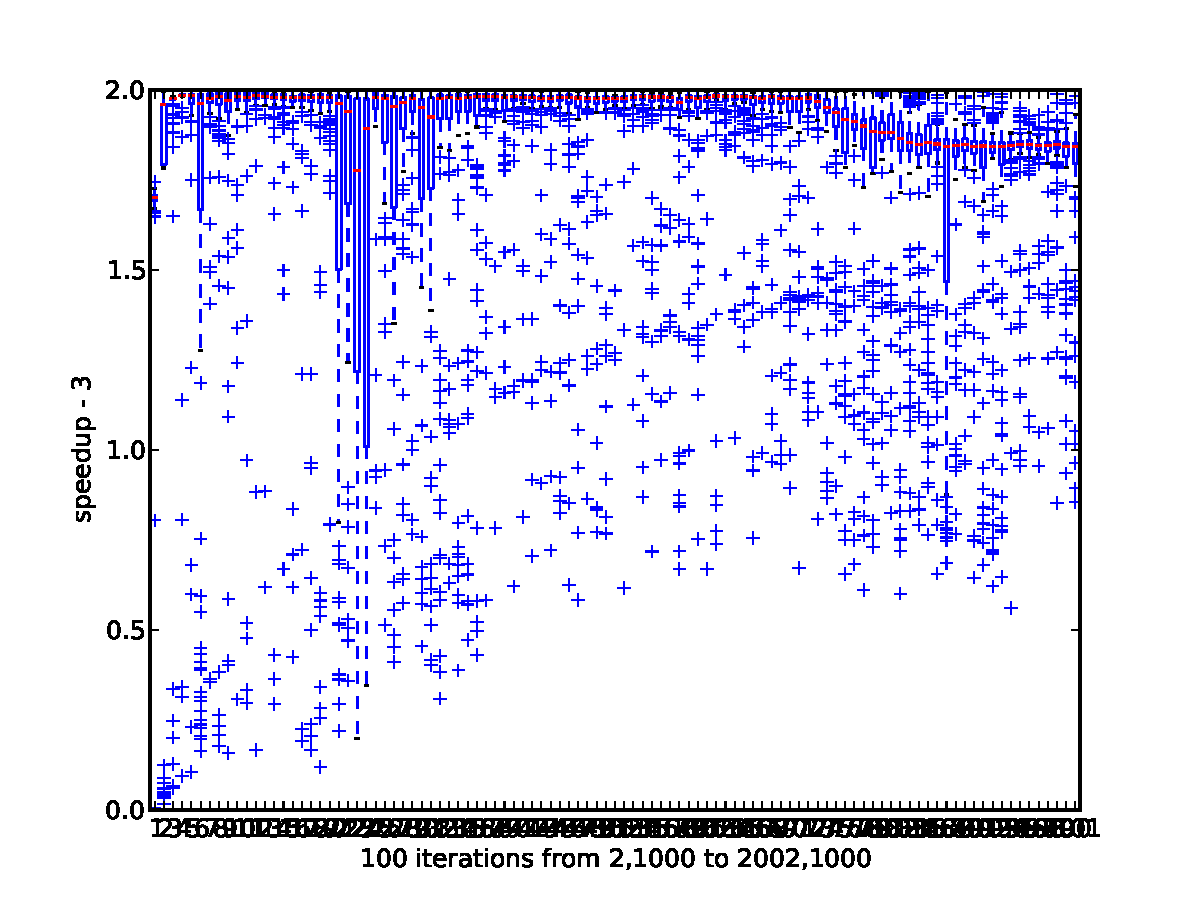
\includegraphics[scale=0.25]{images/openmp_measures_for_2_cores_n2_3_speedup_p2_pS20_P2002_d1000_dS1_D1000_r100_s1.pdf}}
\subfloat[dynamicité sur 2 coeurs]{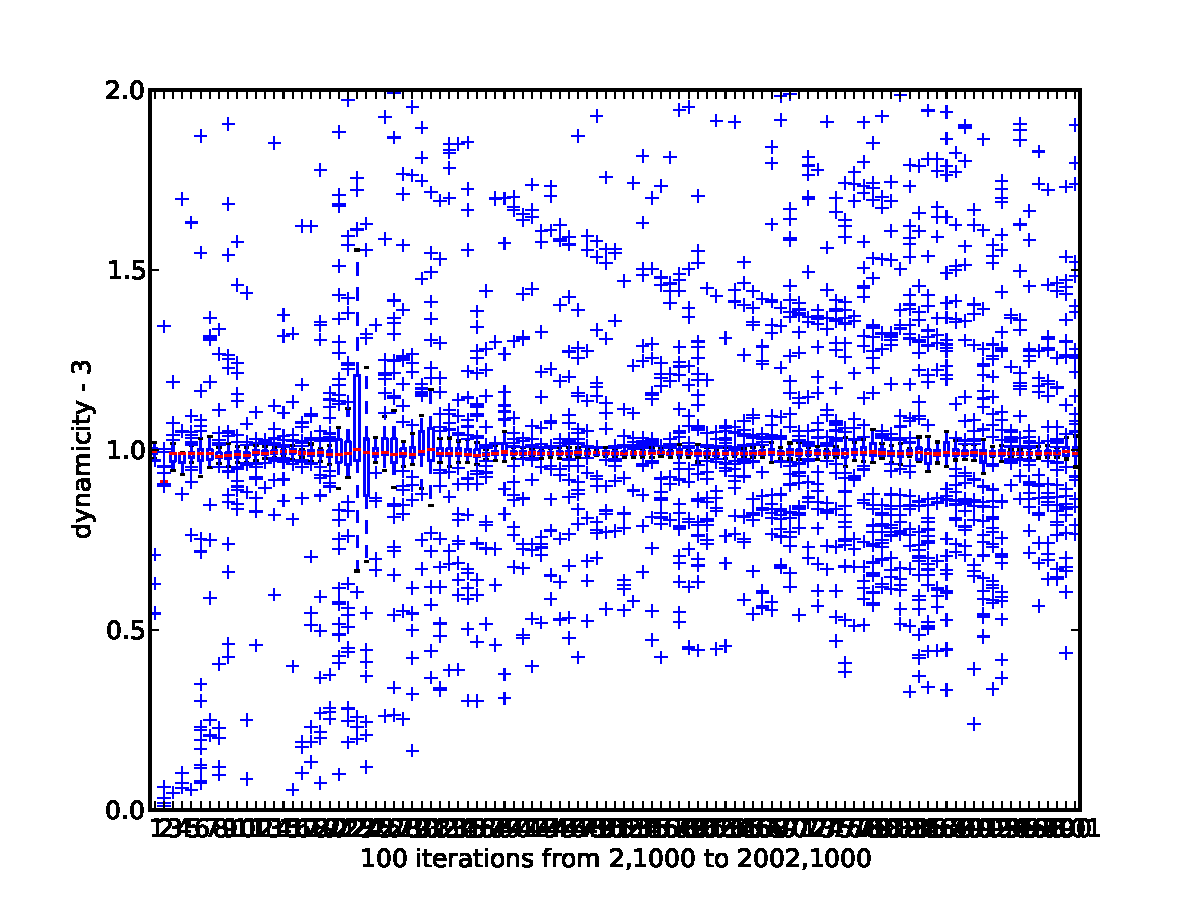
\includegraphics[scale=0.25]{images/openmp_measures_for_2_cores_n2_3_dynamicity_p2_pS20_P2002_d1000_dS1_D1000_r100_s1.pdf}}
\qquad
\subfloat[speedup sur 8 coeurs]{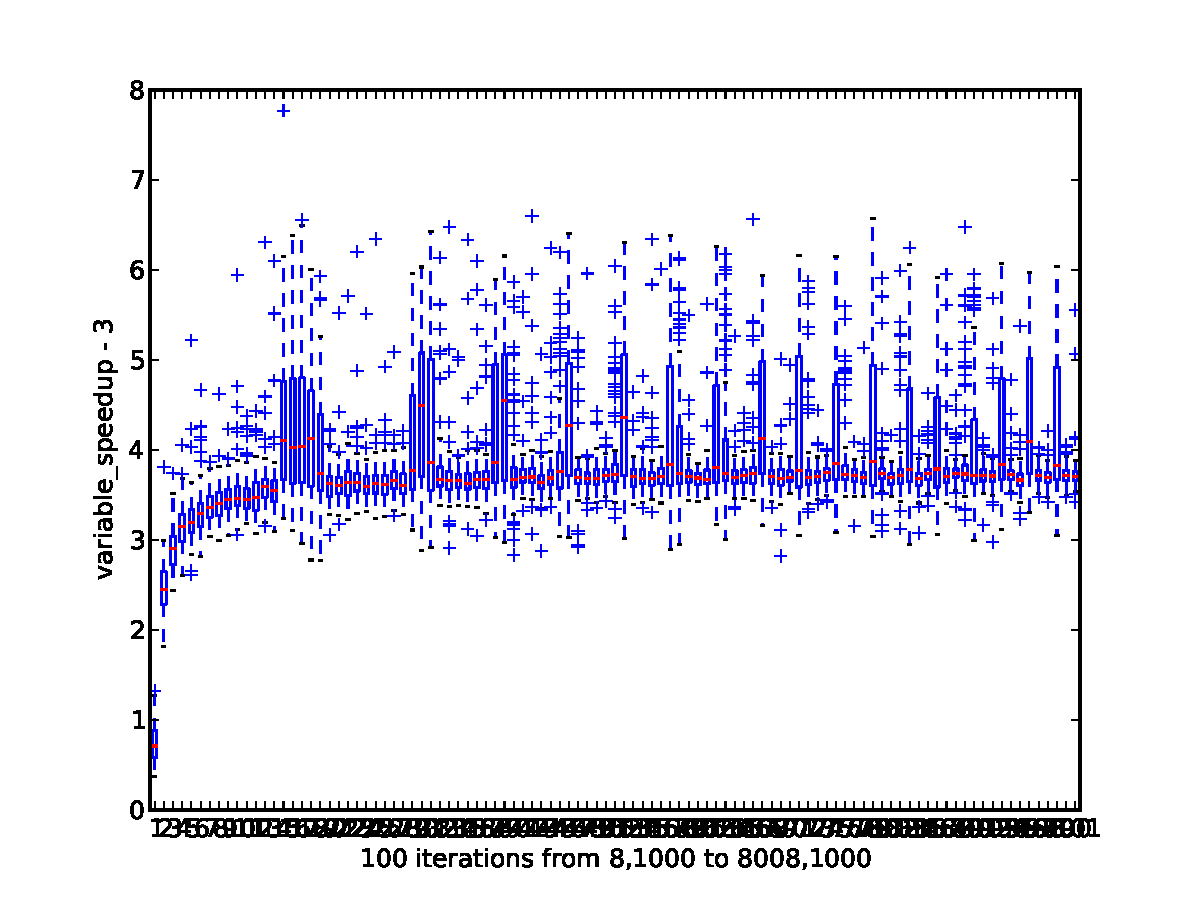
\includegraphics[scale=0.25]{images/openmp_measures_for_8_cores_n8_no_consttime_3_variable_speedup_p8_pS80_P8008_d1000_dS1_D1000_r100_s1.pdf}}
\subfloat[dynamicité sur 8 coeurs]{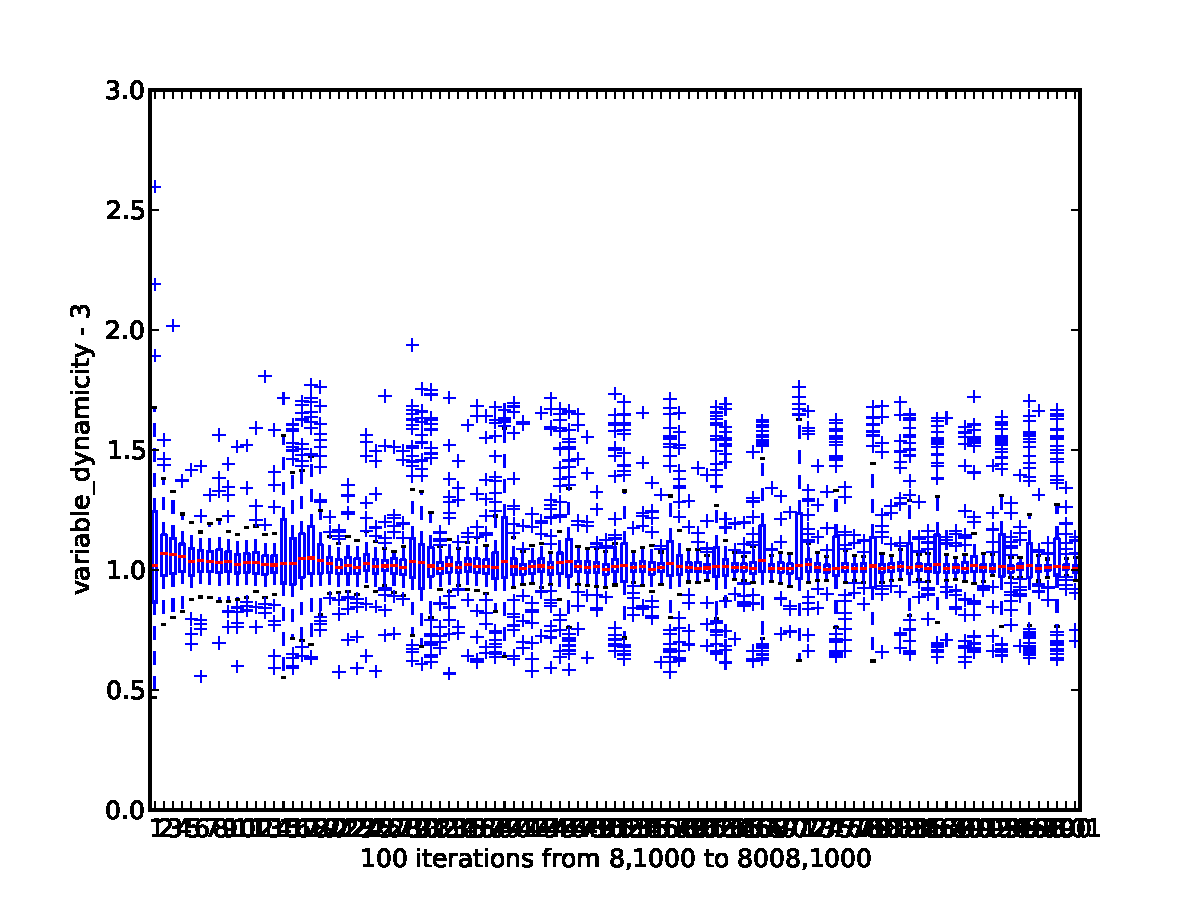
\includegraphics[scale=0.25]{images/openmp_measures_for_8_cores_n8_no_consttime_3_variable_dynamicity_p8_pS80_P8008_d1000_dS1_D1000_r100_s1.pdf}}
\caption{Mesure 3 en $O(n)$ sur 2 et 8 coeurs}
\label{fig:mesure_3_variable}
\end{figure}

\section{Conclusion}

Pour un processeur à 2 coeurs, selon la complexité du problème utilisée, nous pouvons observer par la mesure du speedup que les ressources sont utilisées au maximum\footnote{cpu-bound} pour de grandes tailles d'échantillon. Les petites tailles d'échantillon restant dominées par une exécution séquentielle.\\

Pour un processeur à 8 coeurs, en hyperthreading, notre première observation consiste à montrer les limites de l'hyperthreading, en effet nous utilisons pas plus de 4 coeurs. Et pour rejoindre ce qui a été dit sur 2 coeurs, un plus grand nombre de petites tailles d'échantillon reste dominée par une exécution séquentielle.\\

La différence entre les deux complexités de problème s'observe dans la mesure de la dynamicité. En effet pour un problème en $O(1)$, la planification statique en OpenMP permet d'avoir une meilleur efficacité de travail tandis que en $O(n)$, la planification dynamique apporte quelque amélioration.\\

Pour résumer nous avons comparé par nos mesures les 2 types de planification de tâches en OpenMP, les 2 complexités de problèmes que nous serons amené à paralléliser et finalement sur 2 types de processeurs différents.\\

Un point que je n'ai pas eu le temps d'éclaircir que j'invite à regarder est l'utilisation de l'auto parallélisation intégré au compilateur GCC\footnote{Automatic Parallelization : \url{http://gcc.gnu.org/wiki/openmp}}. Il s'agit d'un niveau d'optimisation qui consiste à vérifier la non dépendance des données dans les boucles et les paralléliser.


% \begin{center}
% \begin{emp}[classdiag](20, 20)
% Class.A("Point")
%        ("+x: int",
%         "+y: int") ();

% Class.B("Circle")
%        ("radius: int")
%        ("+getRadius(): int",
%         "+setRadius(r: int):void");

% topToBottom(45)(A, B);

% drawObjects(A, B);

% clink(aggregationUni)(A, B)
% \end{emp}
% \end{center}

\end{empfile}

% \bibliographystyle{plain}
% \bibliography{references}

\end{document}
